\chapter{The MicroBooNE Experiment}
\label{ch:microboone}

This chapter describes the technical details of the MicroBooNE experiment. Section~\ref{sec:bnb} describes the primary beamline from which MicroBooNE receives neutrinos: the \acrfull{bnb}. Details of the MicroBooNE \acrshort{lartpc} detector are then shown in Section~\ref{sec:detector}.
A comprehension of how a \acrshort{lartpc} works is crucial for understanding the results of the data analysis described in later chapters. This specific detector technology gives rise to certain backgrounds  which are relevant to MicroBooNE measurements and not for other experiments that use different detection techniques. Additionally, the knowledge of the neutrino beamline and the detector operation is precursory to the implementation of the neutrino flux and detector modelling uncertainties that affect the analysis presented in the next chapters. Sections~\ref{sec:trigger},~\ref{sec:readout_data_format},~\ref{sec:simulation} and~\ref{sec:detector_operations} will describe details of the trigger, readout electronics, simulation and detector operations, respectively.


\section{The Booster Neutrino Beamline}
\label{sec:bnb}

\begin{figure}[]
\centering
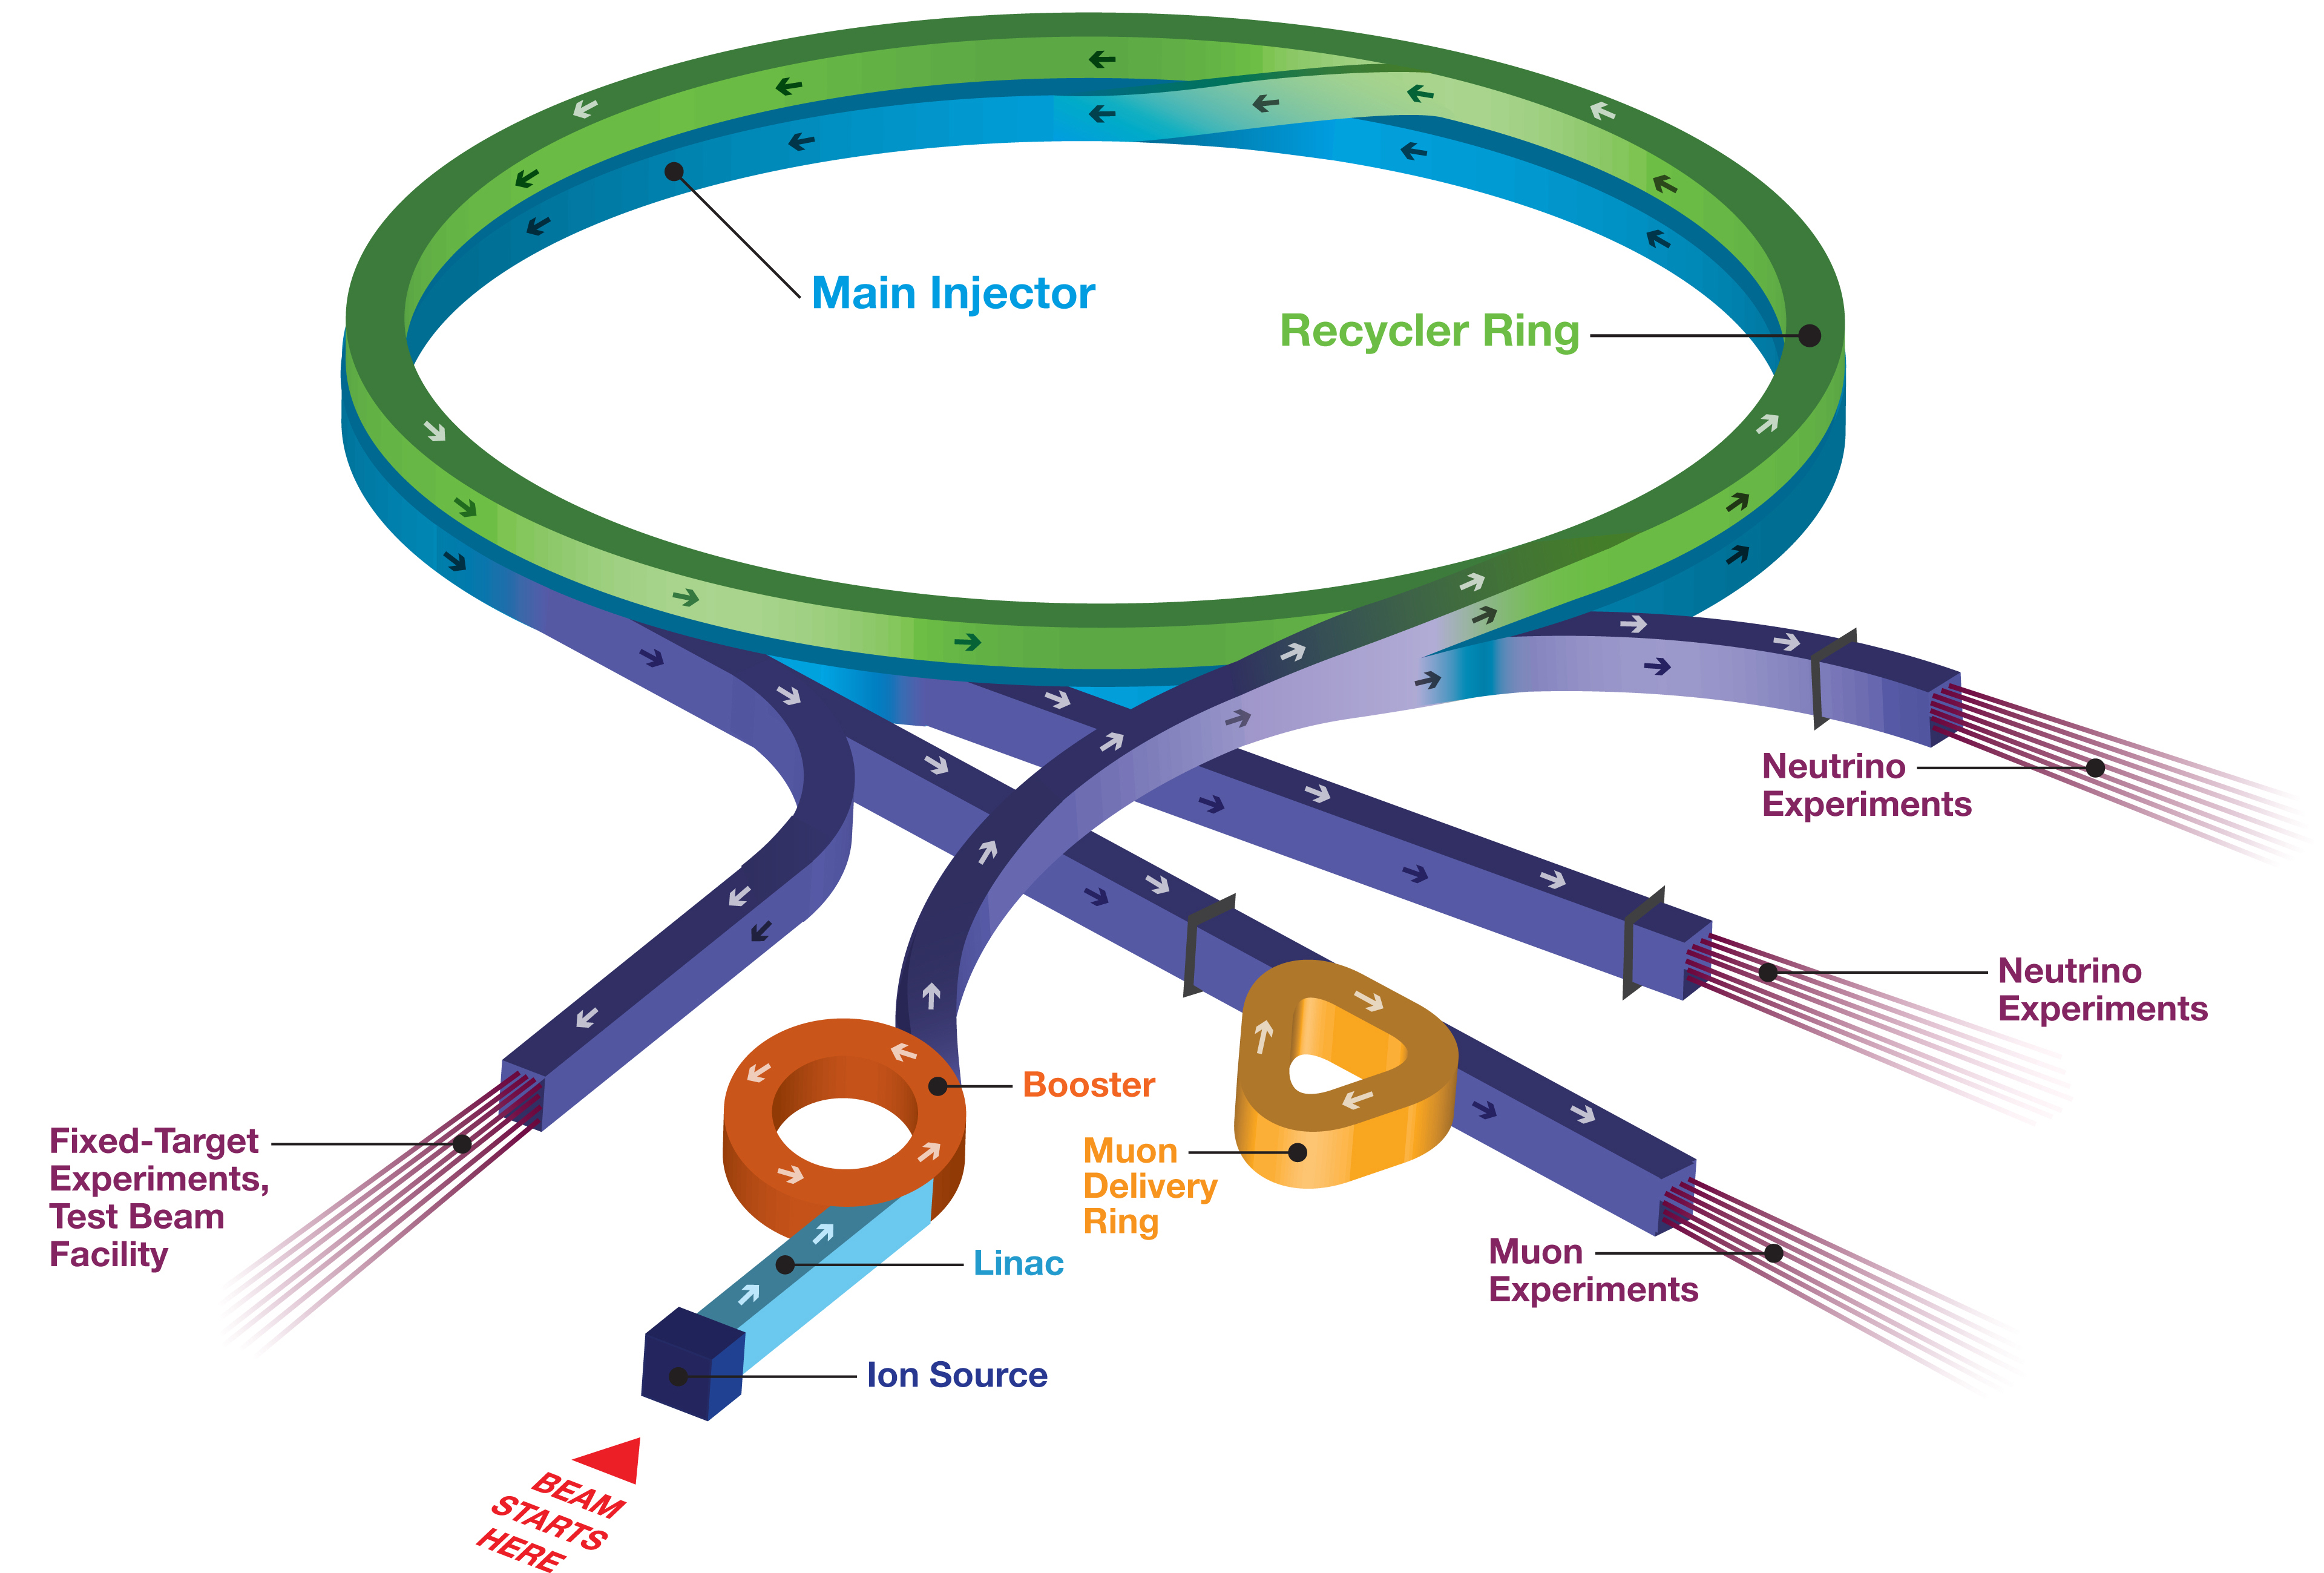
\includegraphics[width=.80\textwidth]{images/MicroBooNE/accelerator-chain}
\caption[Fermilab Accelerator Complex]{The Fermilab accelerator complex. Image source: \cite{doe}.}
\label{fig:accelerator-chain}
\end{figure}

The neutrino beam received by the MicroBooNE experiment is produced at the Fermi National Accelerator Laboratory (Fermilab) thanks to the Fermilab accelerator complex.
This complex, shown in Figure~\ref{fig:accelerator-chain}, is composed of four accelerators that work in tandem \cite{doe}: the linear accelerator (Linac), the Booster, the Recycler, and the Main Injector. These accelerators produce two primary proton beams, a low energy ($8$ GeV) proton beam from the Booster and a high-energy ($120$ GeV) beam from the Main Injector. Hitting a target, these proton beams produce secondary beams of pions, kaons, muons and neutrinos that serve a variety of experiments.
 
This section describes in some detail the production process of neutrinos through the \acrshort{bnb} beamline. Three sections will describe the main stages involved: the production and extraction of an 8 GeV proton beam, in Section~\ref{sec:beam}; the beam target and focusing horn which lead to a secondary meson beam, in Section~\ref{sec:target}; and the composition of the neutrino beam reaching the MicroBooNE detector, in Section~\ref{sec:composition}.


%NuMI is a tertiary beam resulting from the decays of pion and kaon secondaries produced in the NuMI target. Protons of $120$ GeV are fast-extracted from the Main Injector (MI) accelerator and bent downward by $58$ mrad toward Soudan, MN. The beam line is designed to accept $4.9 \times 10^{13}$ protons per pulse (ppp). The repetition rate is $0.75$ Hz, giving about $6\times 10^{20}$ protons on target per year, \cite{tdr}.

\subsection{Primary Proton Beam}
\label{sec:beam}

The Booster proton beam starts as a beam of negatively charged hydrogen ions $H^-$. The  $H^-$ ions are subjected to a linear accelerator using alternating electromagnetic fields that accelerate them to 400 MeV kinetic energy \cite{miniboone_flux}.
Electrons are removed from the $H^-$ ions through a carbon foil. The bare protons enter the 474-meter-circumference Booster synchrotron, which operates at a frequency of 15 Hz. Here, the protons are accelerated up to 8.89 GeV momentum. The protons are bunched in ``beam spills'' containing roughly $4 \times 10^{12}$ protons spaced throughout a 1.6 $\mu$s time window per spill. The protons are then directed toward a thick beryllium target.

The absolute number of \acrfull{pot} is measured by two toroids upstream of the target which are part of a larger beam monitoring system. The uncertainty on the \acrshort{pot} is on the order of 2\% \cite{miniboone_flux}. Additional beam characteristics are monitored by beam position monitors, a multi-wire chamber, and a resistive wall monitor.  This system measures beam intensity, timing, width, position, and direction of the proton beam.


\subsection{Beam Target and Focusing Horn}
\label{sec:target}

The beryllium target hit by the protons is made up of seven identical cylindrical segments of beryllium, to produce a cylinder 71.1 cm long and 0.51 cm in radius. These are contained within a sleeve (1.37 cm inner radius, 0.9 cm thickness) also made of beryllium, which is connected to each segment via three beryllium fins. The volume of air within the sleeve is circulated to provide cooling for the target.

When the protons hit the target, secondary particles are produced, including pions and kaons, which represent the primary source of neutrinos and anti-neutrinos. 
To enhance the neutrino beam, these secondaries are focused by a toroidal electromagnet (horn) placed around the target. 
Inside the horn, a toroidal magnetic field provides a restoring force for particles of a certain charge, and defocuses particles of the opposite charge, thus enhancing a $\nu_\mu$ beam while reducing $\bar{\nu}_\mu$ background (or vice versa) originating from the decay of the secondary particles. The more focused the mesons are before the decay, the more focused will the neutrino beam be once it reaches the detector, enhancing the flux. 
The focusing horn is made of aluminium and is pulsed with a 174 kA current. A drawing of the horn structure is shown in Figure~\ref{fig:horn}. 
\begin{figure}[]
\centering
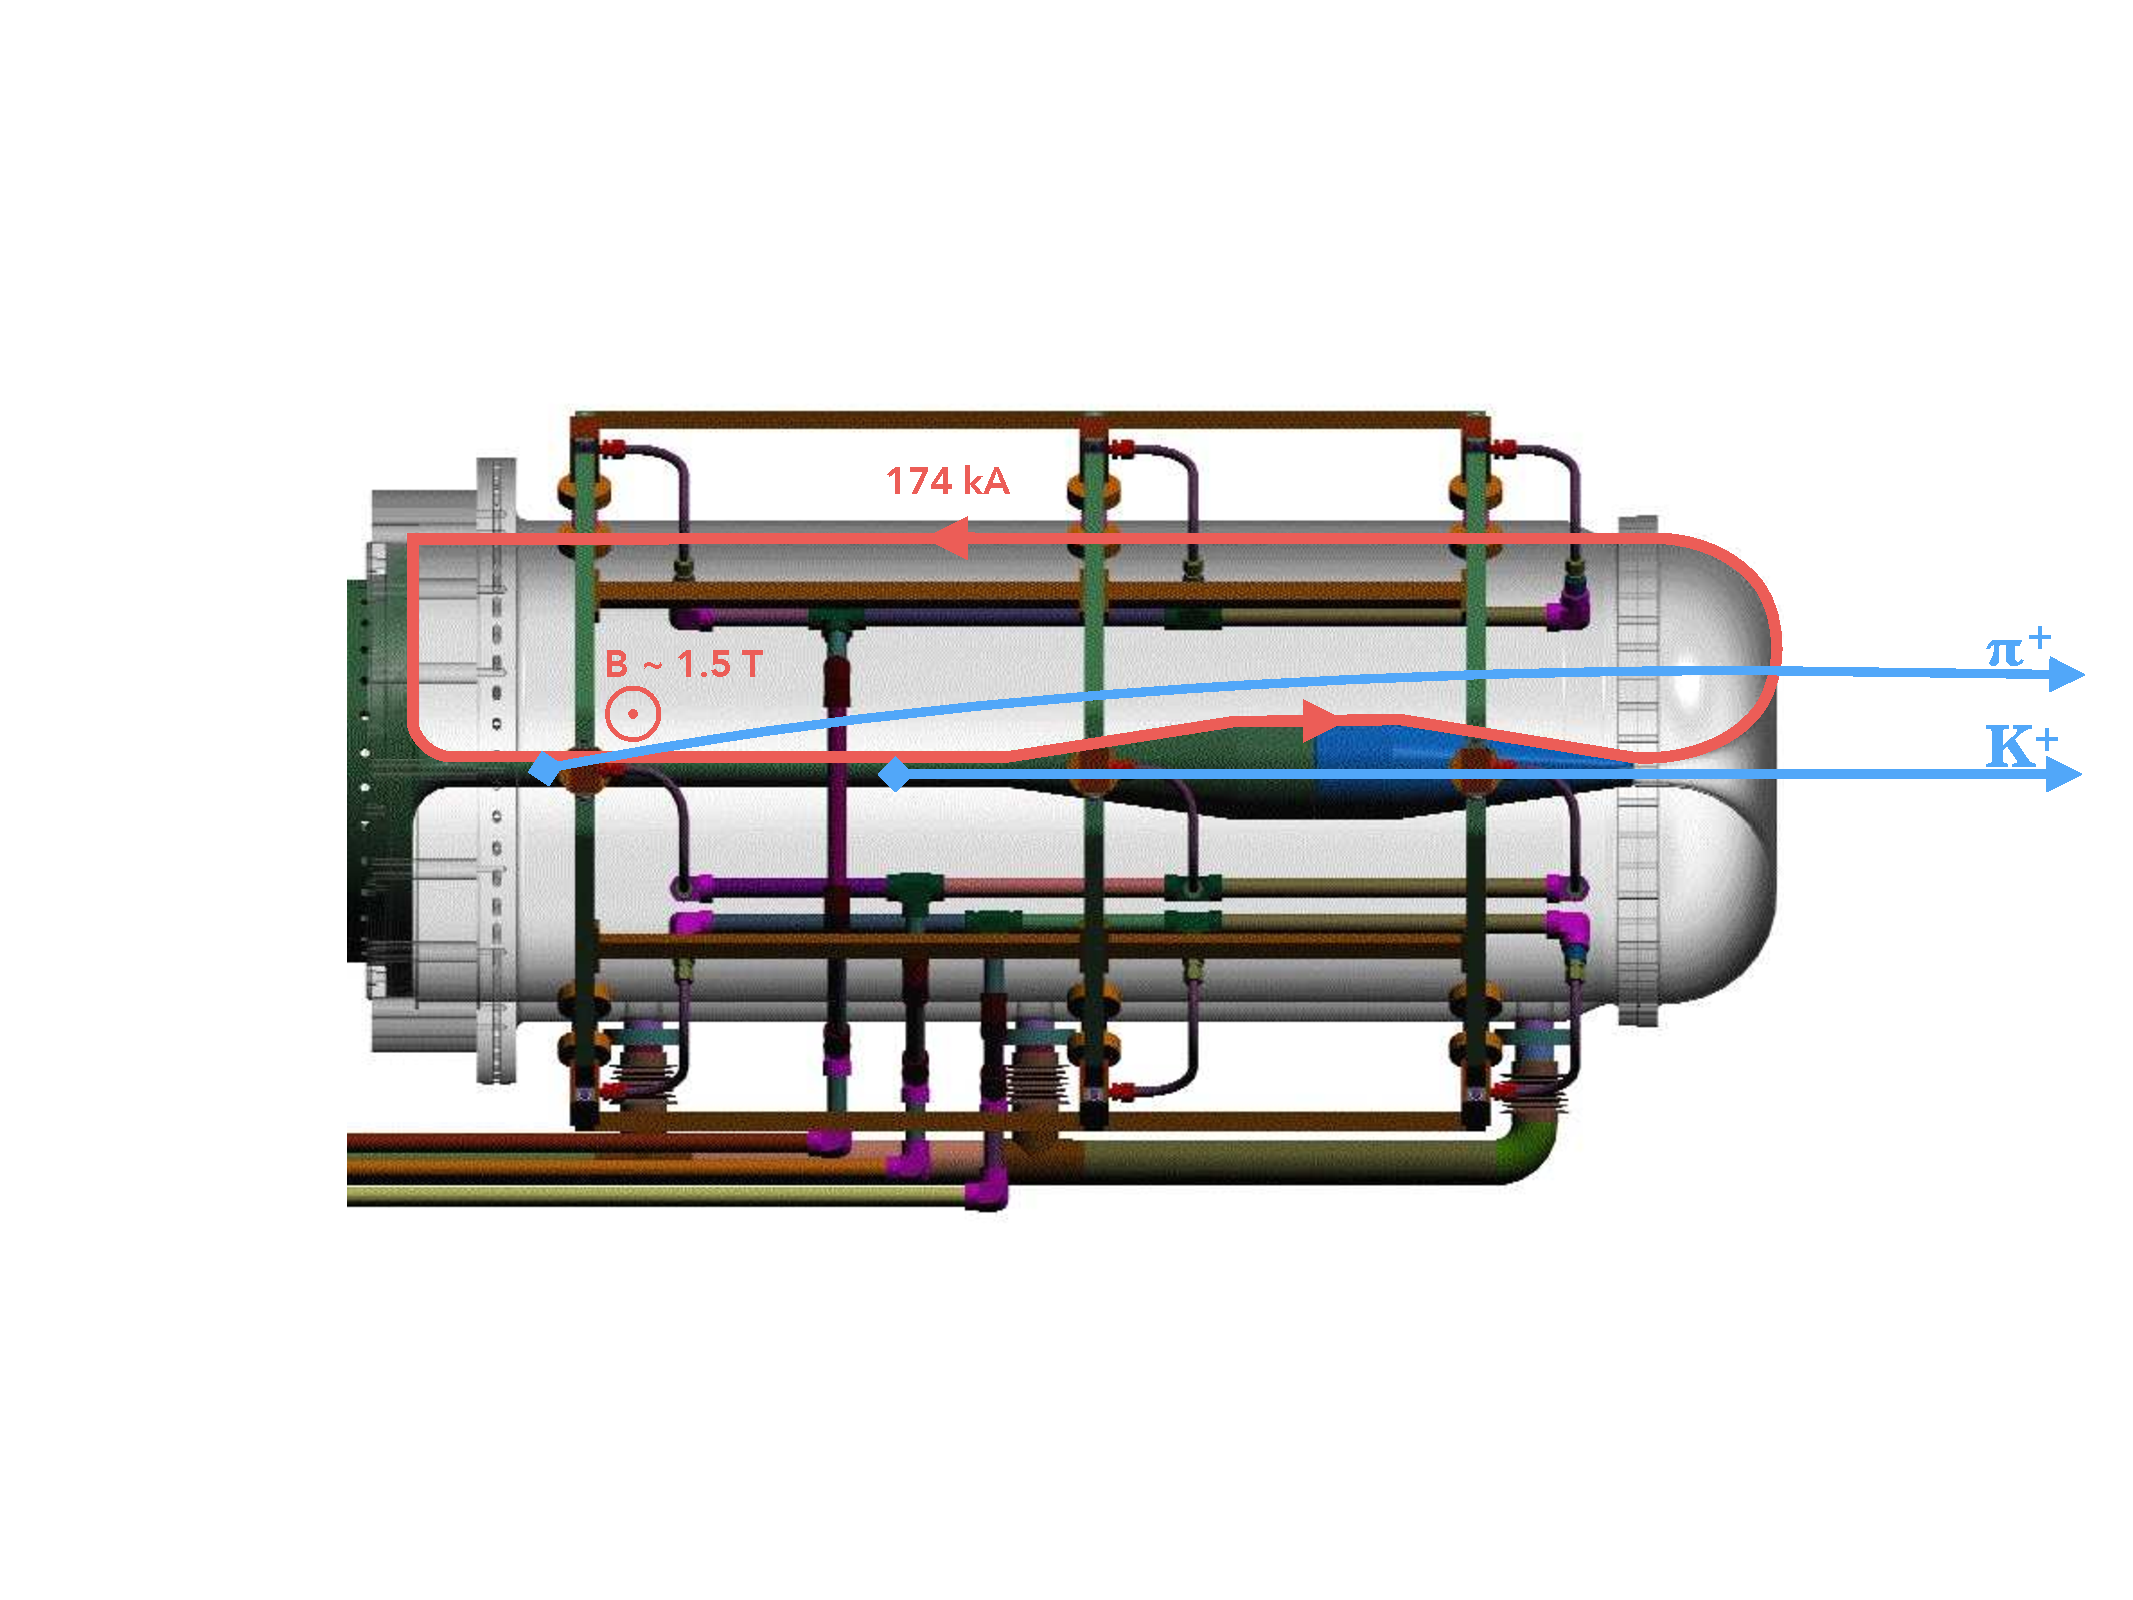
\includegraphics[width=.80\textwidth]{images/MicroBooNE/horn}
\caption[MiniBooNE Horn]{The pulsed horn system. The outer conductor (grey) is transparent to show the inner conductor components running along the centre (dark green and blue). The target assembly is inserted into the inner conductor from the left side. In neutrino-focusing mode, the (positive) current flows from left-to-right along the inner conductor, returning along the outer conductor. The plumbing associated with the water cooling system is also shown. Adapted from \cite{miniboone_flux}.}
\label{fig:horn}
\end{figure}
The horn is 185 cm long and is composed of an inner and outer conducting cylinders. A positive current travels down the inner conductor, and arches back towards the front via the outer conductor, producing a magnetic field perpendicular to the beam direction within its volume and falls off as $1/r$. The inner conductor is placed just outside the beryllium target. Right outside the inner conductor, the strength of the magnetic field reaches 1.5 Tesla. Since the horn heats up due to the pulsed current and radiation, during running the inner conductor is being cooled with nozzles that spray water on it.
The direction of the current can be switched to focus the positively charged secondaries (as shown in Figure~\ref{fig:horn}), or the negatively charged secondaries, ultimately producing a beam primarily of  neutrinos (``neutrino mode'') or antineutrinos (``antineutrino mode''), respectively. 
The \acrshort{bnb} beamline is schematically shown in Figure~\ref{fig:bnb}.
The horn has a small field-free region, called the neck of the horn. The particles can pass through that region without being affected. The neck also allows the remaining proton beam to go through, without hitting the horn.
%A concrete collimator is located downstream of the target/horn assembly to absorb particles that would not otherwise contribute to the neutrino flux.

Focused charged pions and kaons travel through a 50-meter decay region: a cylindrical volume of air, in which pions and kaons decay, producing the tertiary neutrino beam which eventually reaches the detector. 
Remaining charged particles which have not yet decayed are blocked by an absorber made of concrete. The absorber stops the hadron component of the beam, while neutrinos and some of the muons pass through it.
By this point, the beam is composed almost entirely of neutrinos which propagate through the dirt before reaching the detector. 

\begin{figure}[]
\centering
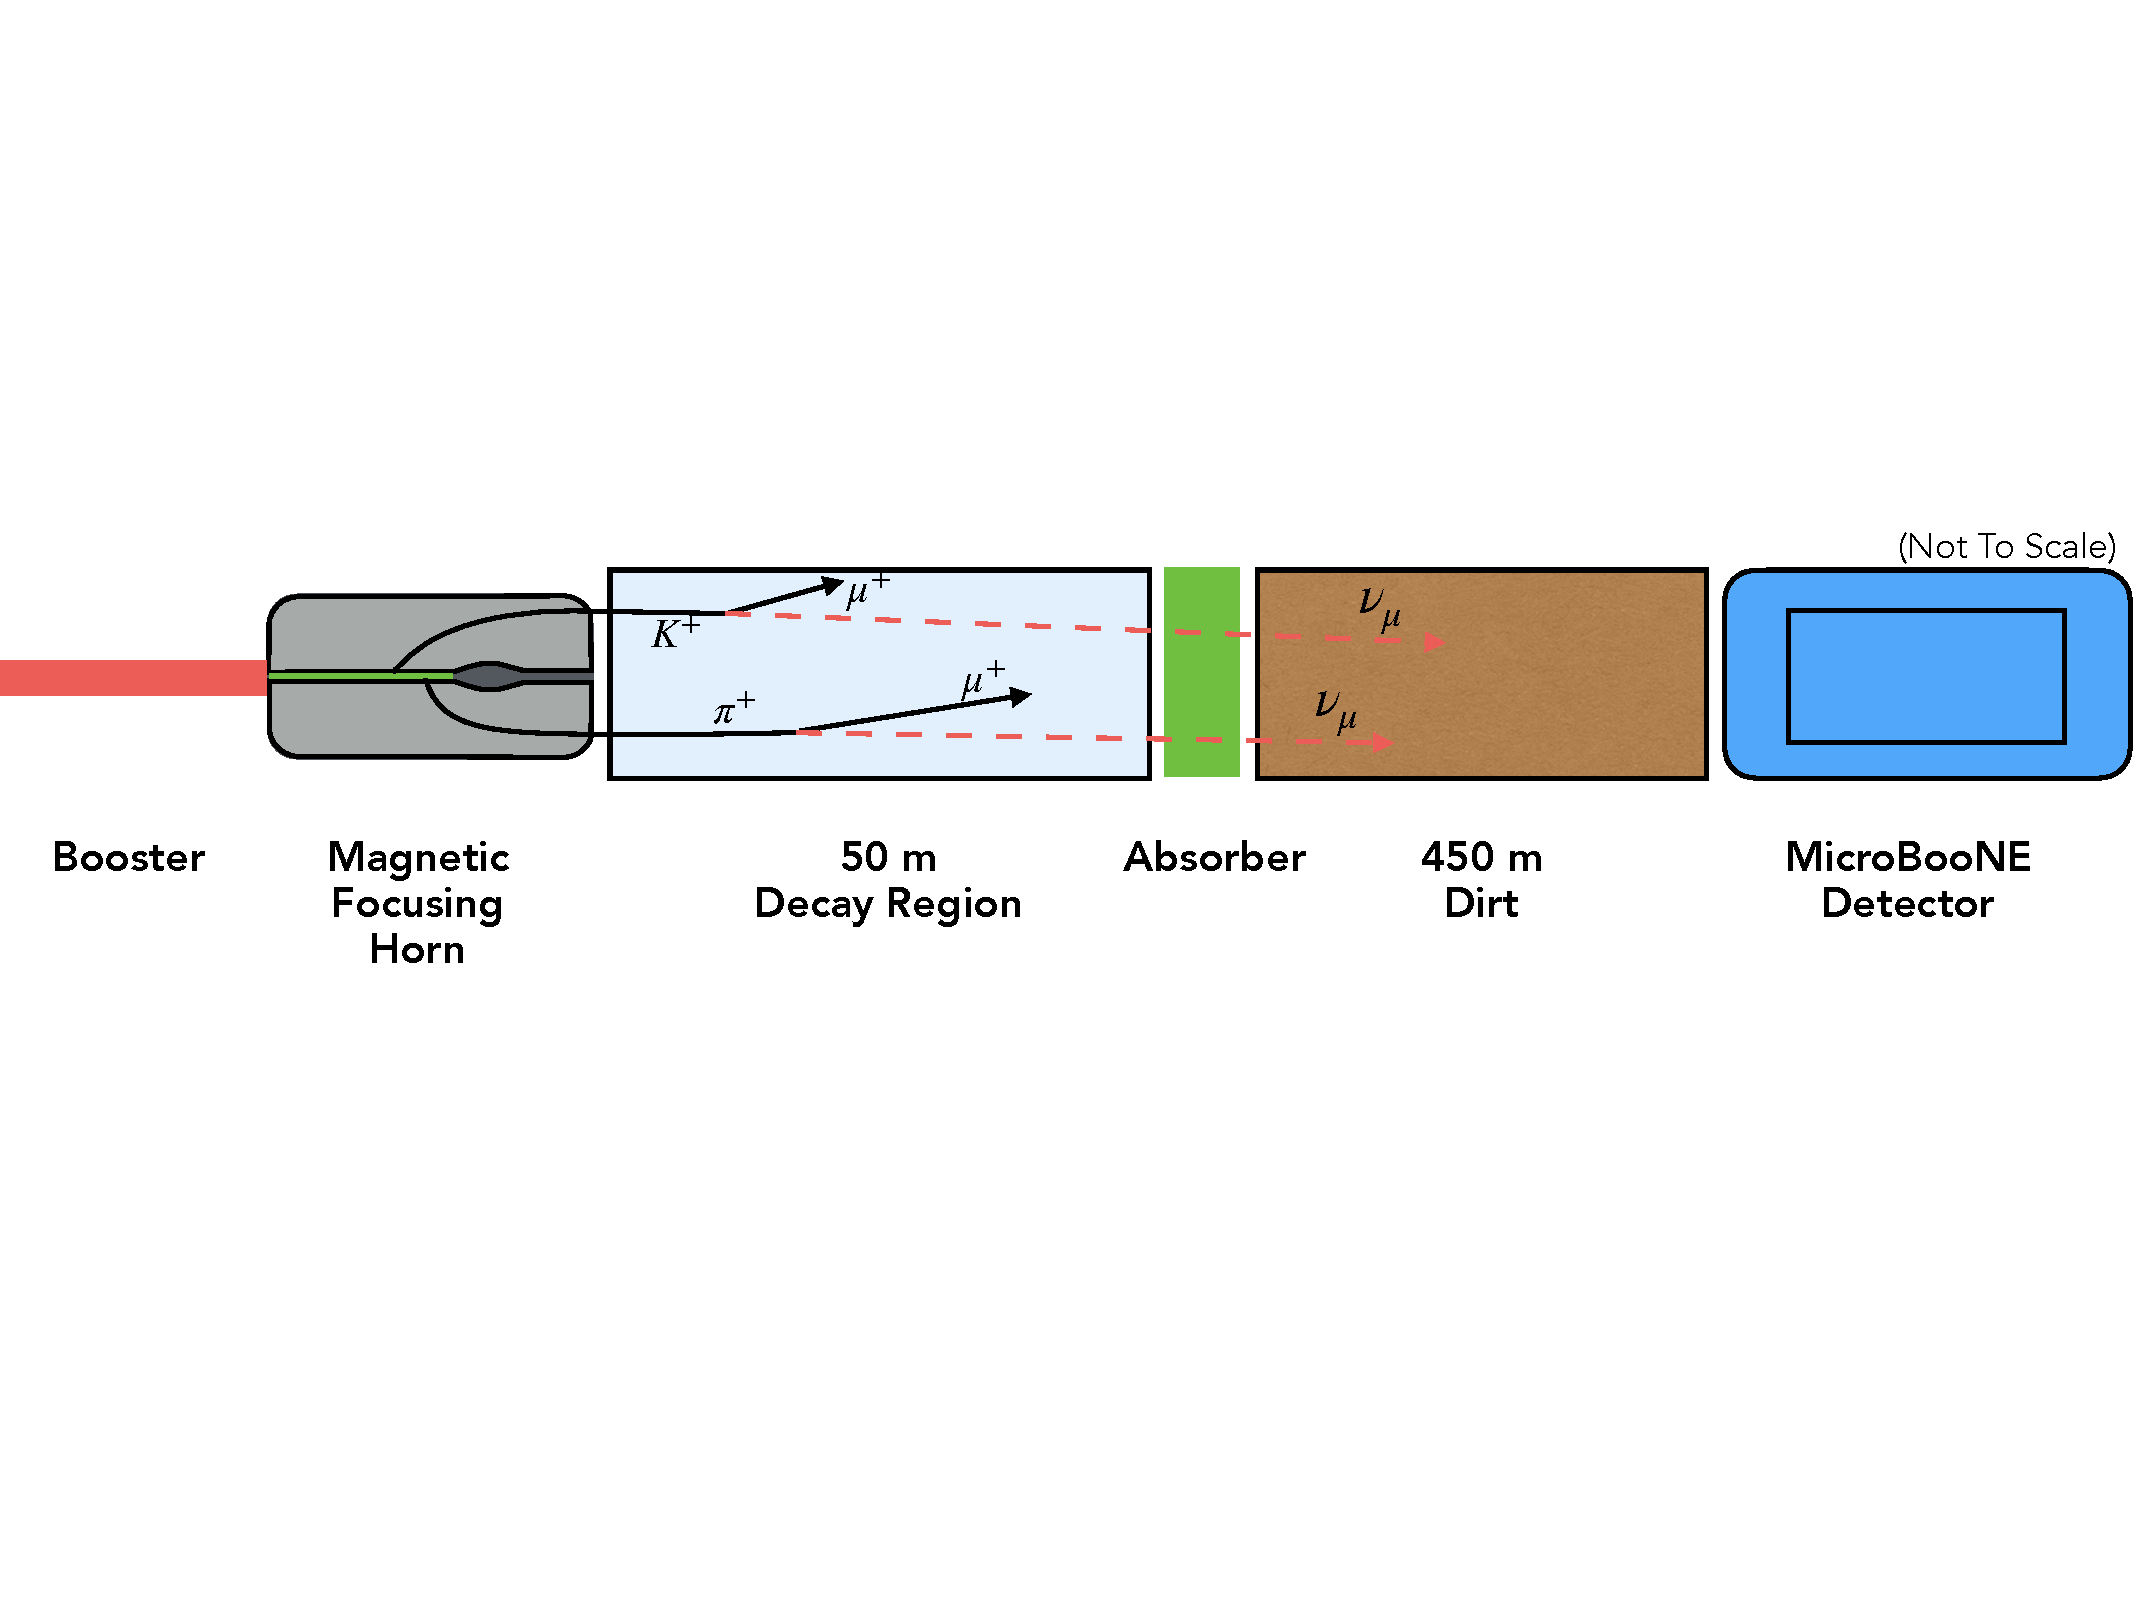
\includegraphics[width=1.0\textwidth]{images/MicroBooNE/bnb}
\caption[Booster Neutrino Beamline]{Schematic of the \acrlong{bnb}.}
\label{fig:bnb}
\end{figure}









\subsection{Beam Composition}
\label{sec:composition}

\begin{figure}[]
\centering
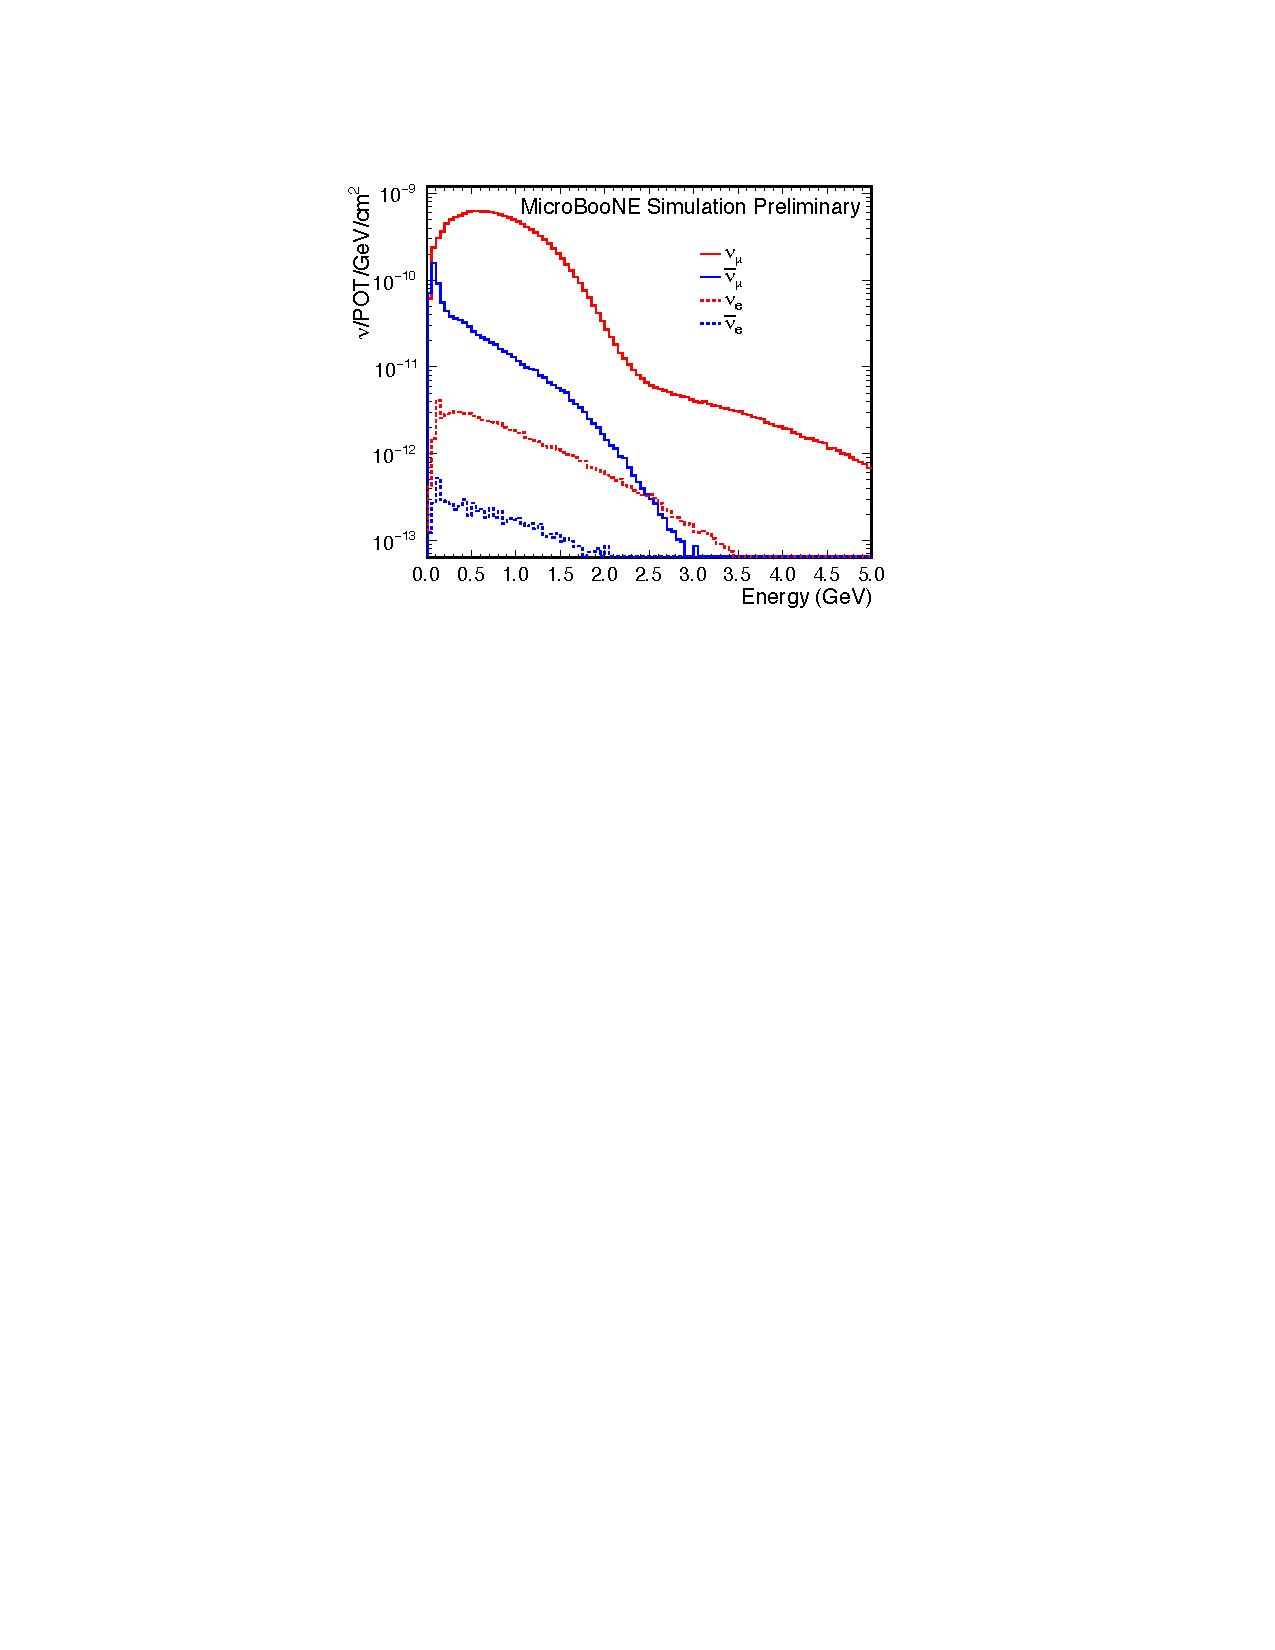
\includegraphics[width=.70\textwidth]{images/MicroBooNE/flux}
\caption[Neutrino Flux Prediction at MicroBooNE]{Neutrino flux prediction at MicroBooNE. Figure from~\cite{flux_note}.}
\label{fig:flux}
\end{figure}

The analysis described in this thesis makes use of a data set collected when the horn was pulsed with a positive current, resulting in positively charged mesons being focused towards the beam axis, while negatively charged were deflected away. 
Pions are the most abundant particles produced in the target, and this results in a $\pi^+$ beam with a small contribution of $K^+$ and $\mu^+$. In the decay region, these secondary particles are left free to decay. Pions predominantly decay in $\mu^+$ and $\nu_\mu$, hence giving rise to the $\nu_\mu$ beam. At the same time, contamination from other neutrino states in pion decay are caused by either $\bar{\nu}_\mu$ or by $\nu_e$ coming from the decay of muons ($\mu^+ \rightarrow e^+ + \bar{\nu}_\mu + \nu_e$). $\bar{\nu}_\mu$ also come from the contamination in the beam from $\mu^-$ which are very forward going or very energetic and therefore are not deflected by the horn.

Neutrinos produced by the decay of kaons ($K^\pm$, $K^0$, $K_L^0$) also contribute to the flux. Due to the smaller kaon production rate in the target this is a minor contribution to the total neutrino flux. Almost the entire flux of $\nu_\mu$ with  energy below 2.5 GeV is contributed by events which originate from pion decay, while kaons contribute almost exclusively to $\nu_\mu$ beyond this energy. Most importantly, because of the broader range of decay channels, kaons contribute significantly to the $\nu_e$ flux, even at lower energies. A small fraction of $\bar{\nu}_e$ also arises from kaon decay.

In the end, the neutrino beam produced at the \acrshort{bnb} is a 93.6\% $\nu_\mu$ beam, with a contamination of $\bar{\nu}_\mu$ (5.86\%), $\nu_e$ (0.52\%) and $\bar{\nu}_e$ (0.05\%). Figure~\ref{fig:flux} shows the neutrino flux split in the contributions from the four neutrino states as modelled by the MiniBooNE beam simulation~\cite{miniboone_flux} and calculated at the MicroBooNE detector.

\section{The MicroBooNE Detector}
\label{sec:detector}

The MicroBooNE detector is located along the \acrshort{bnb} beamline, 470 m from the target.
It is a 60 metric ton fiducial mass (170 metric ton total mass) \acrshort{lartpc} detector \cite{det}, contained within a cylindrical cryostat, where charged particles traversing a volume of highly-purified liquid argon leave trails of ionisation electrons along their paths, and also create prompt ultraviolet scintillation photons. Ionisation electrons drift in an electric field to a system of three anode wire planes. Waveforms originate from drift electrons inducing signals on the three wire planes, as shown in Figure~\ref{fig:tpc}. The MicroBooNE \acrfull{tpc} is described in Section~\ref{sec:tpc}.
The scintillation photons are observed by \acrshort{pmt}s located behind the wire planes, described in Section~\ref{sec:pmt}.




\subsection{Time Projection Chamber}
\label{sec:tpc}

\begin{figure}[]
\centering
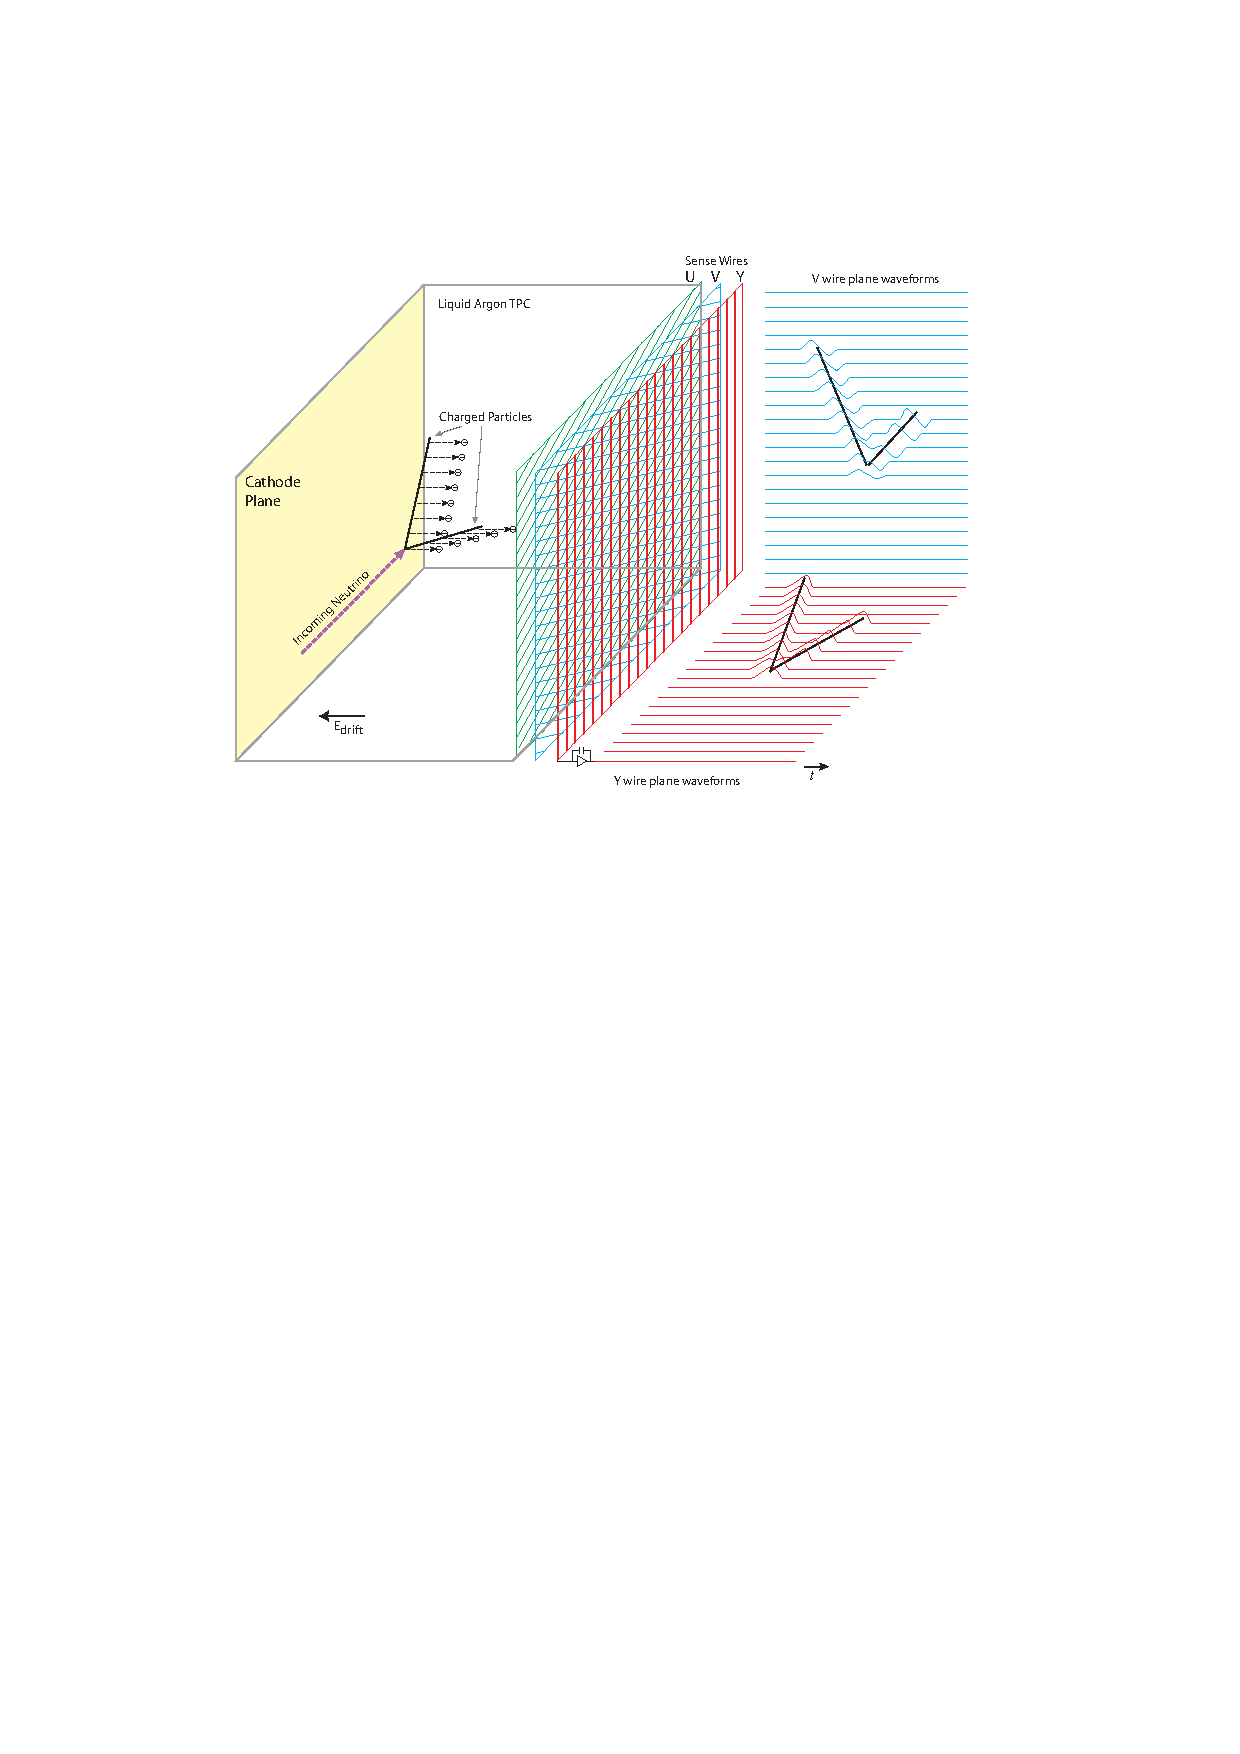
\includegraphics[width=.90\textwidth]{images/MicroBooNE/tpc}
\caption[MicroBooNE Time Projection Chamber]{Operational principle of the MicroBooNE \acrshort{lartpc}. Ionisation electrons from particles traversing the detector medium are drifted by an electric field past multiple planes of sense wires. The signals on those wires create several two-dimensional images of the event and can be combined to obtain a three-dimensional view of the event. \acrshort{pmt}s are also used to collect scintillation light, but are not drawn in this diagram. Image source:~\cite{det}.}
\label{fig:tpc}
\end{figure}

\begin{figure}[t]
\centering
\subfloat[][]
   {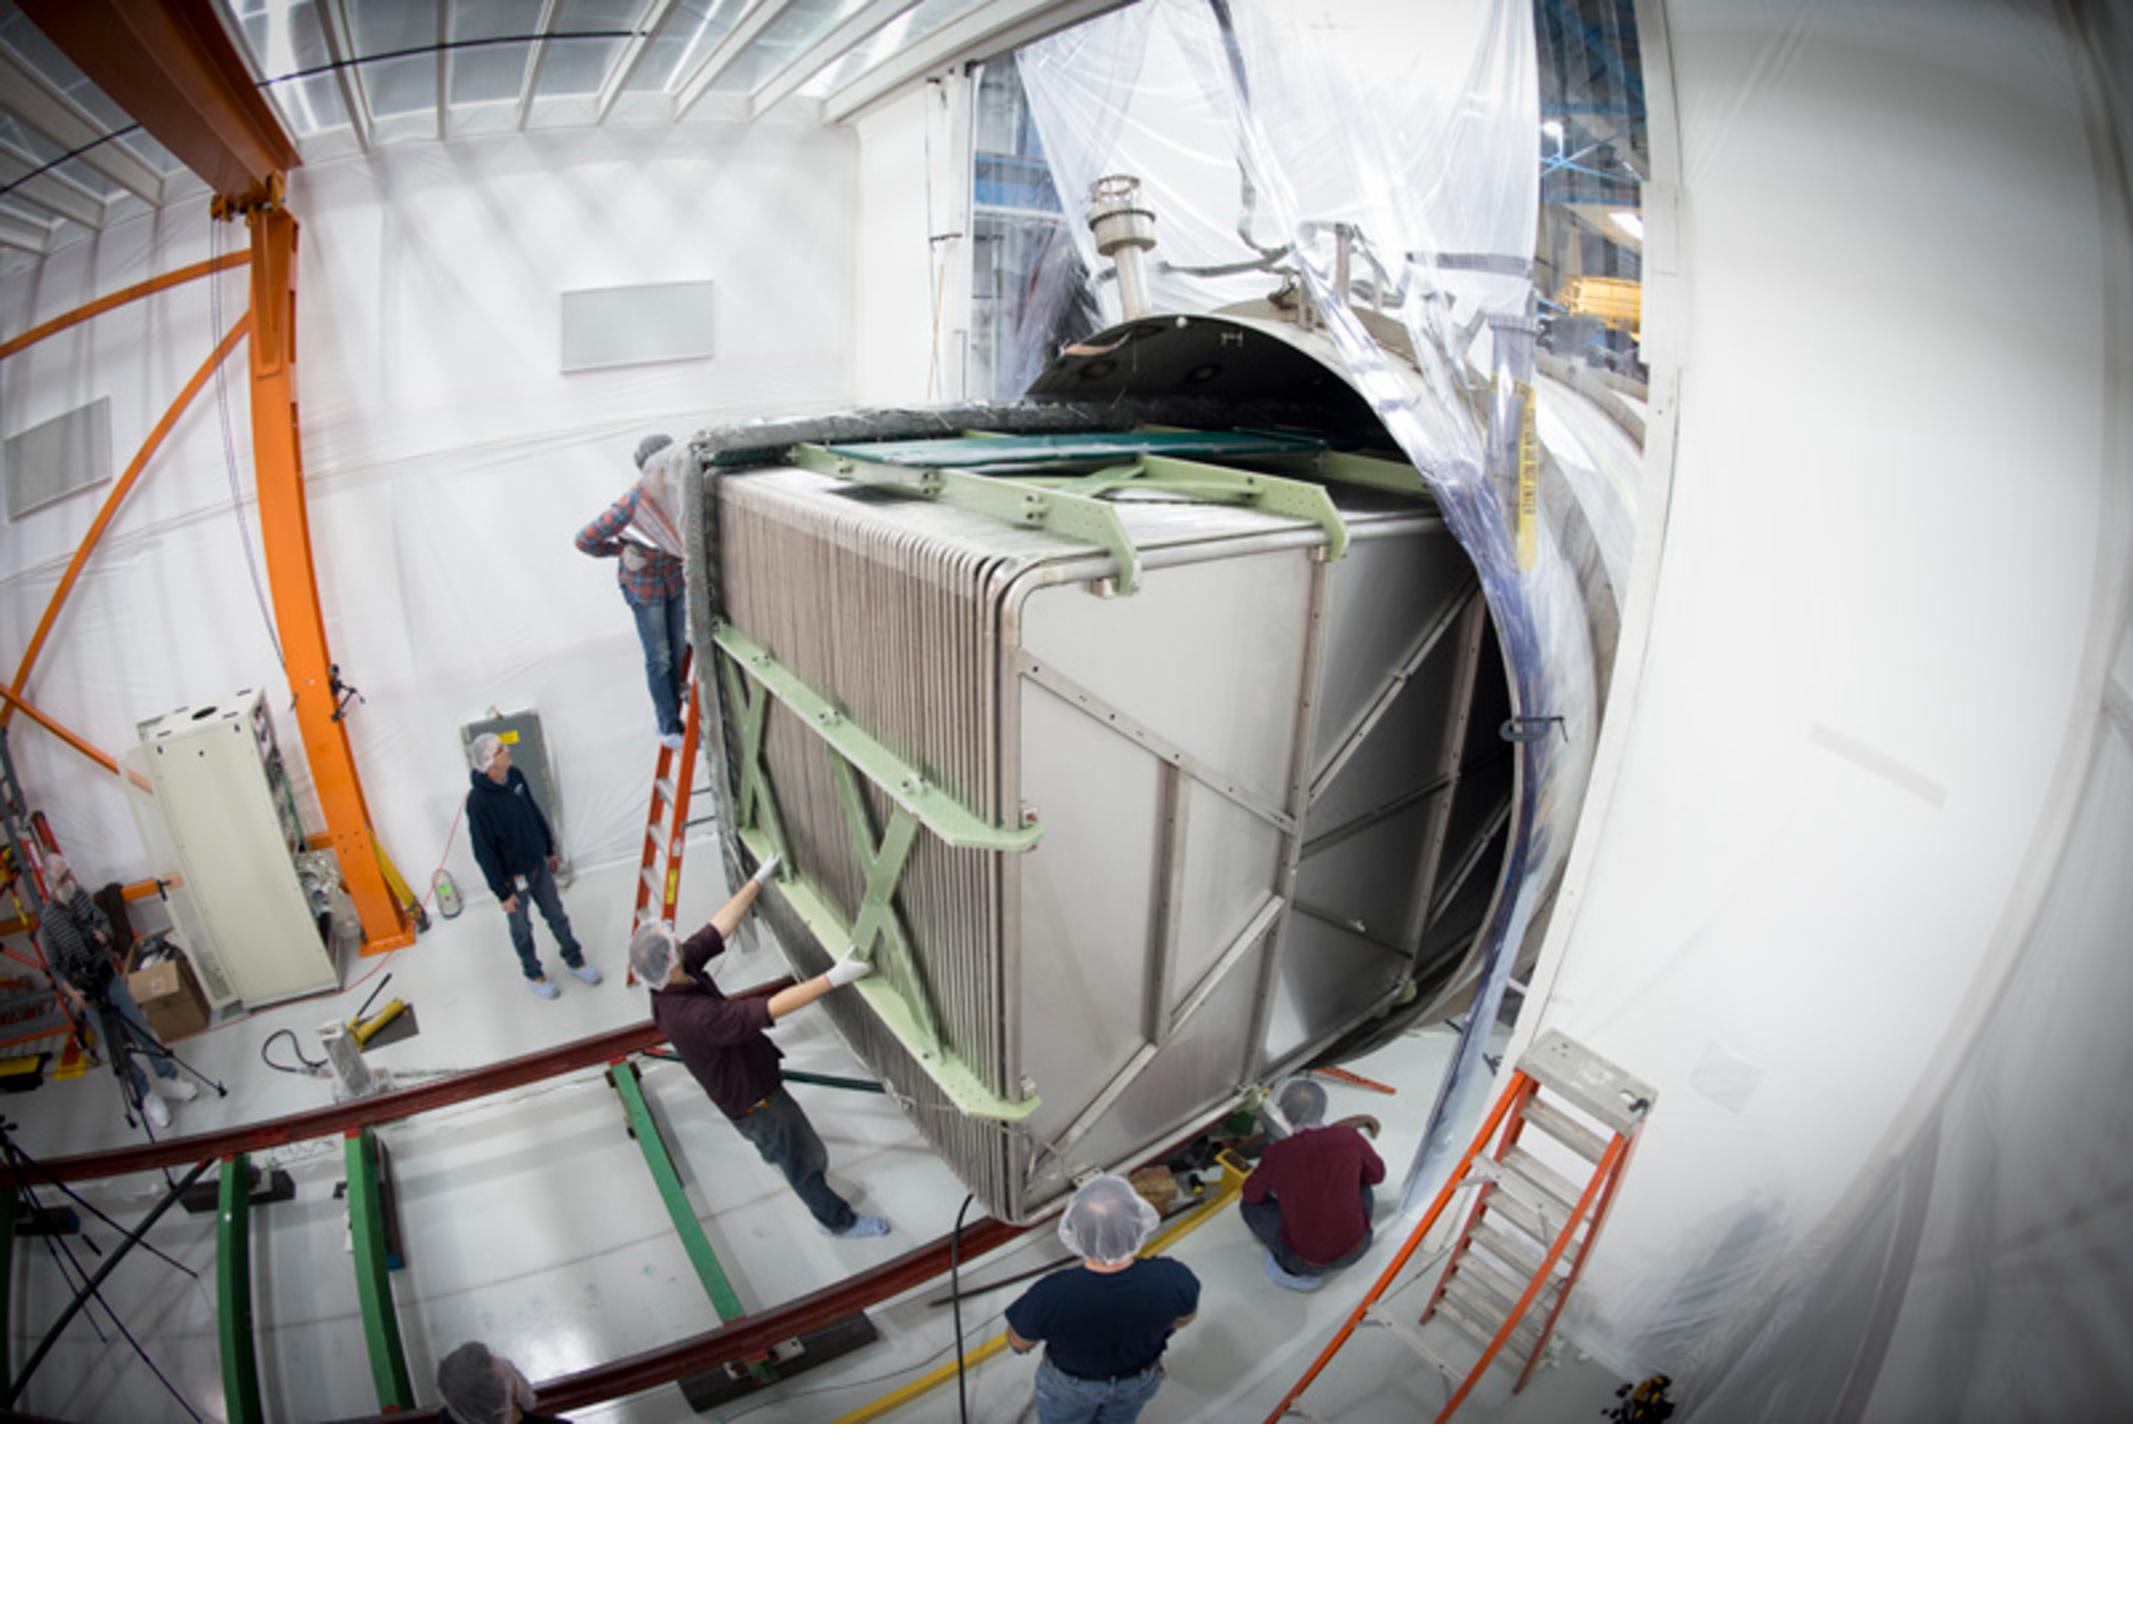
\includegraphics[width=.48\textwidth]{images/MicroBooNE/det_pic_1}
   \label{fig:det_pic_1}} 
\subfloat[][]
   {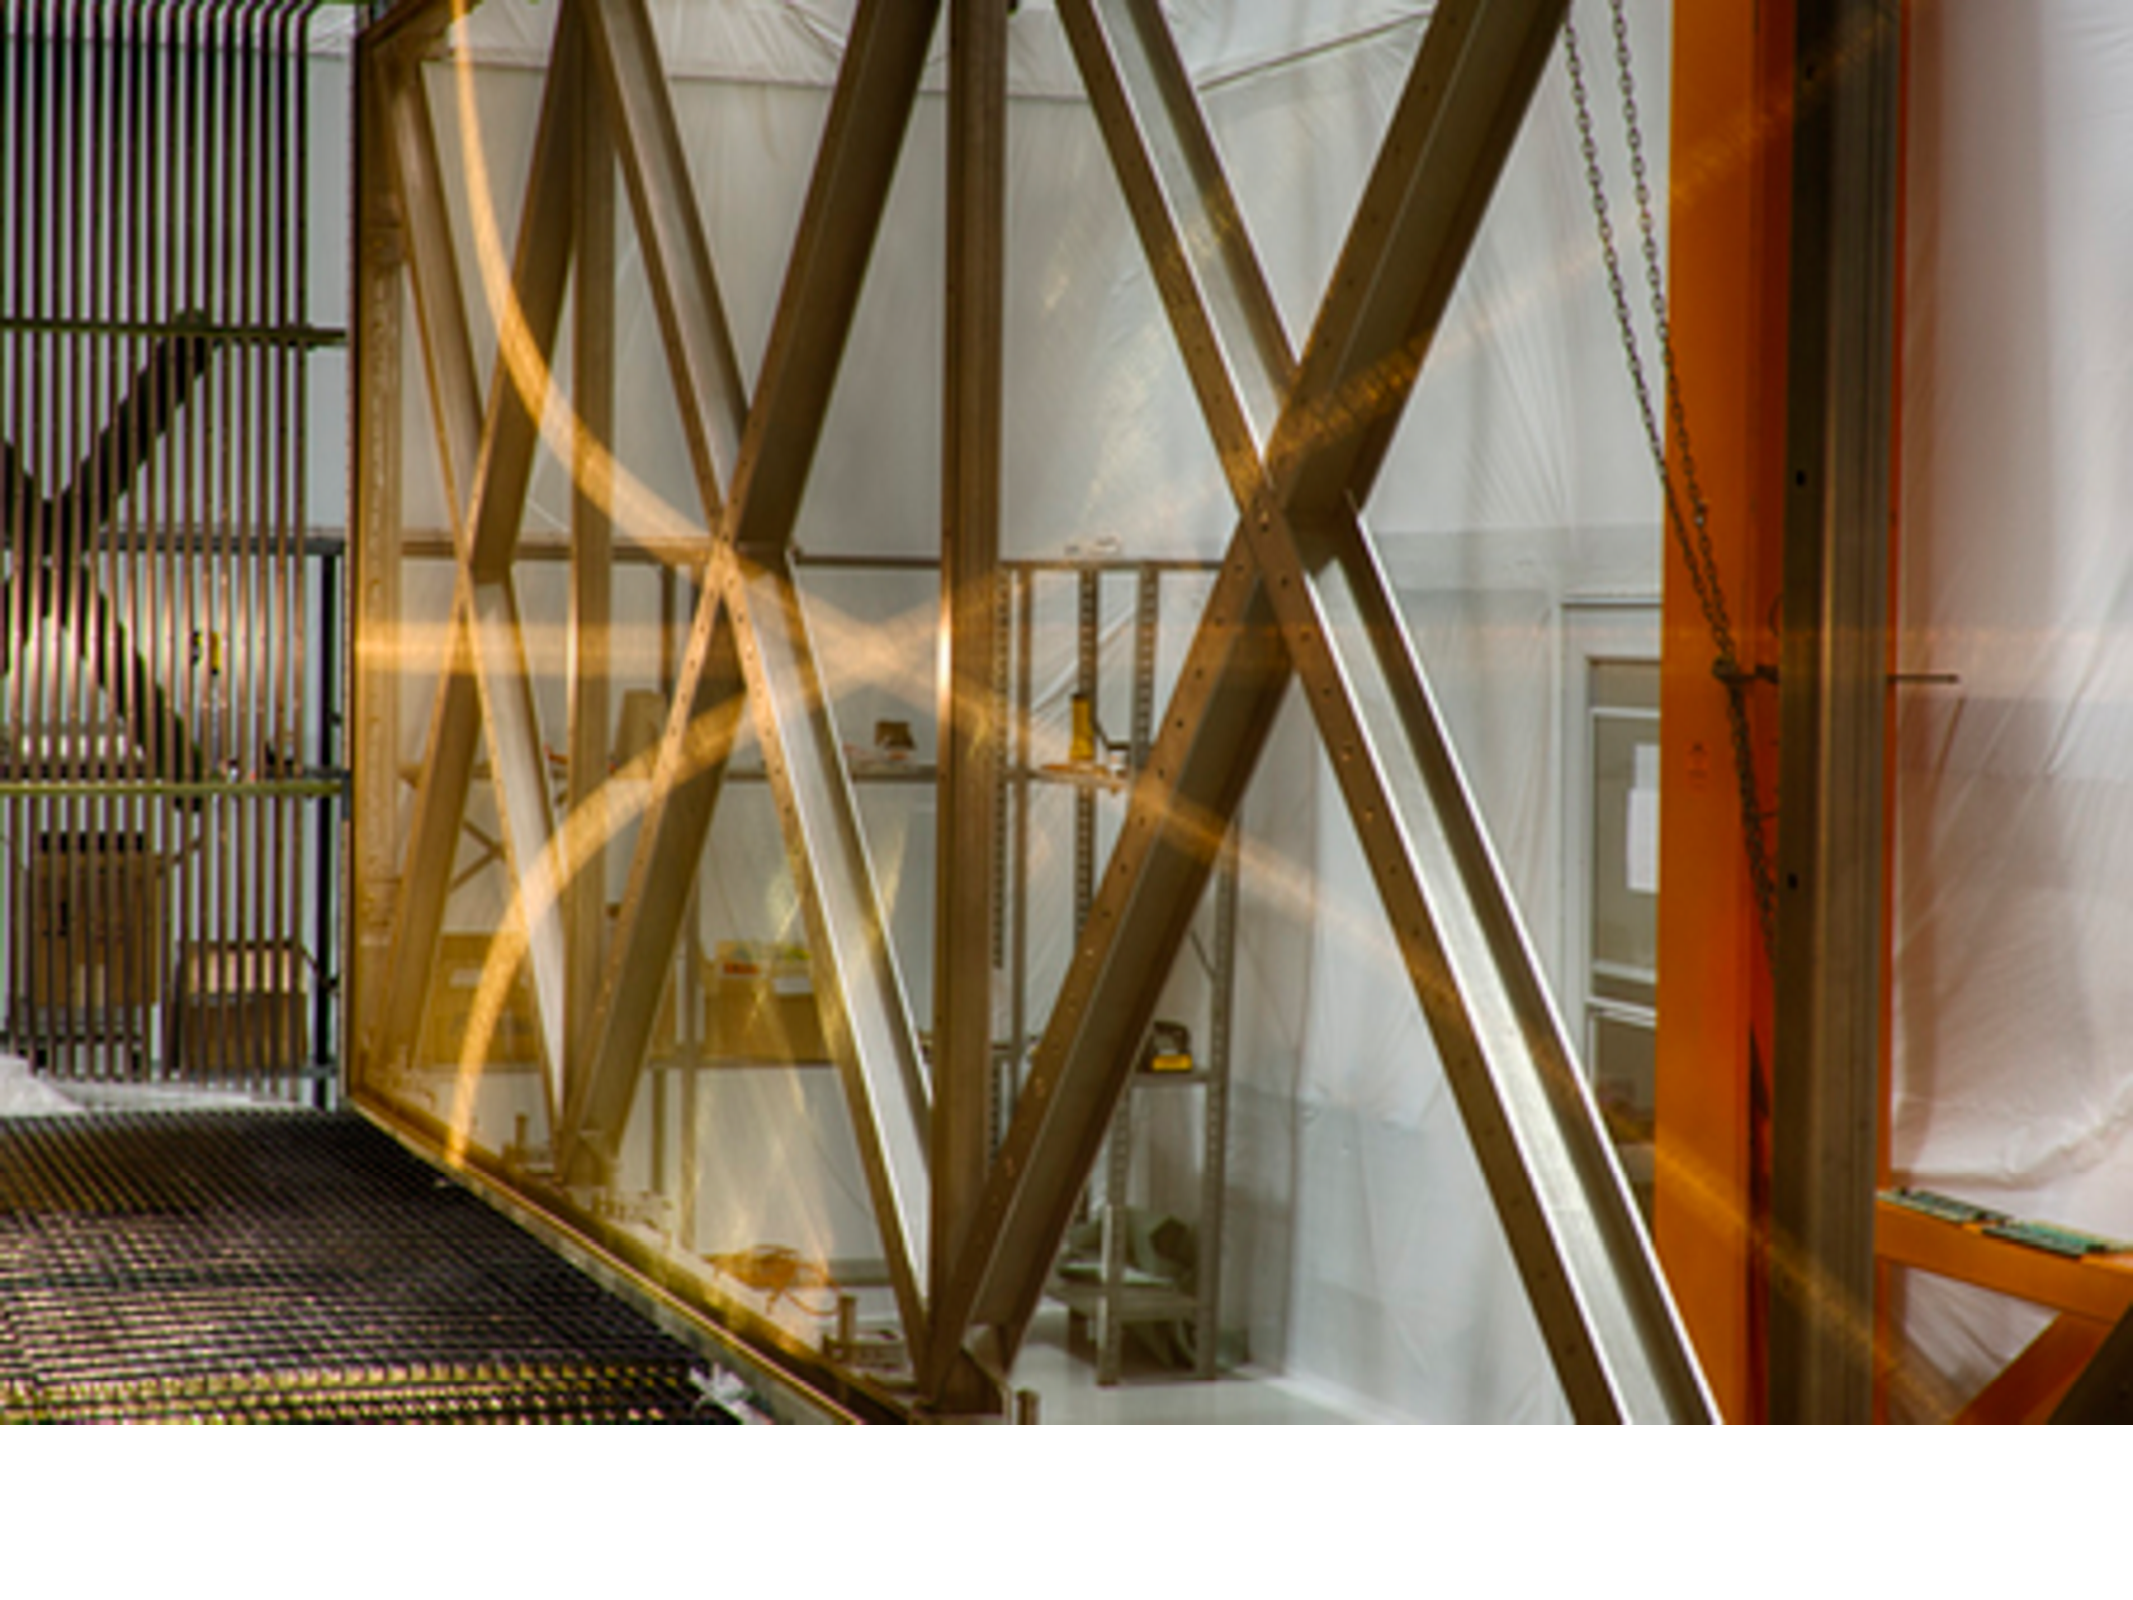
\includegraphics[width=.48\textwidth]{images/MicroBooNE/det_pic_2}
   \label{fig:det_pic_2}}
\caption[MicroBooNE Detector Pictures]{The MicroBooNE \acrshort{tpc} when it was inserted in the cryostat~\protect\subref{fig:det_pic_1}. The cathode is visible on the front right and the field cage, made of tubes, can also be seen. The inside the \acrshort{tpc}~\protect\subref{fig:det_pic_2}. The three wire planes are visible along the anode on the right, and the field cage tubes at the back.}
\label{fig:det_pic}
\end{figure}

The \acrshort{tpc} used in the MicroBooNE experiment, shown in Figure~\ref{fig:det_pic}, is a rectangular parallelepiped with dimensions 2.3 m (height) $\times$ 2.6 m (width) $\times$ 10.4 m (length, along the beam direction). The coordinate system adopted is shown in Figure~\ref{fig:tpc_coordinates}. 
\begin{figure}[]
\centering
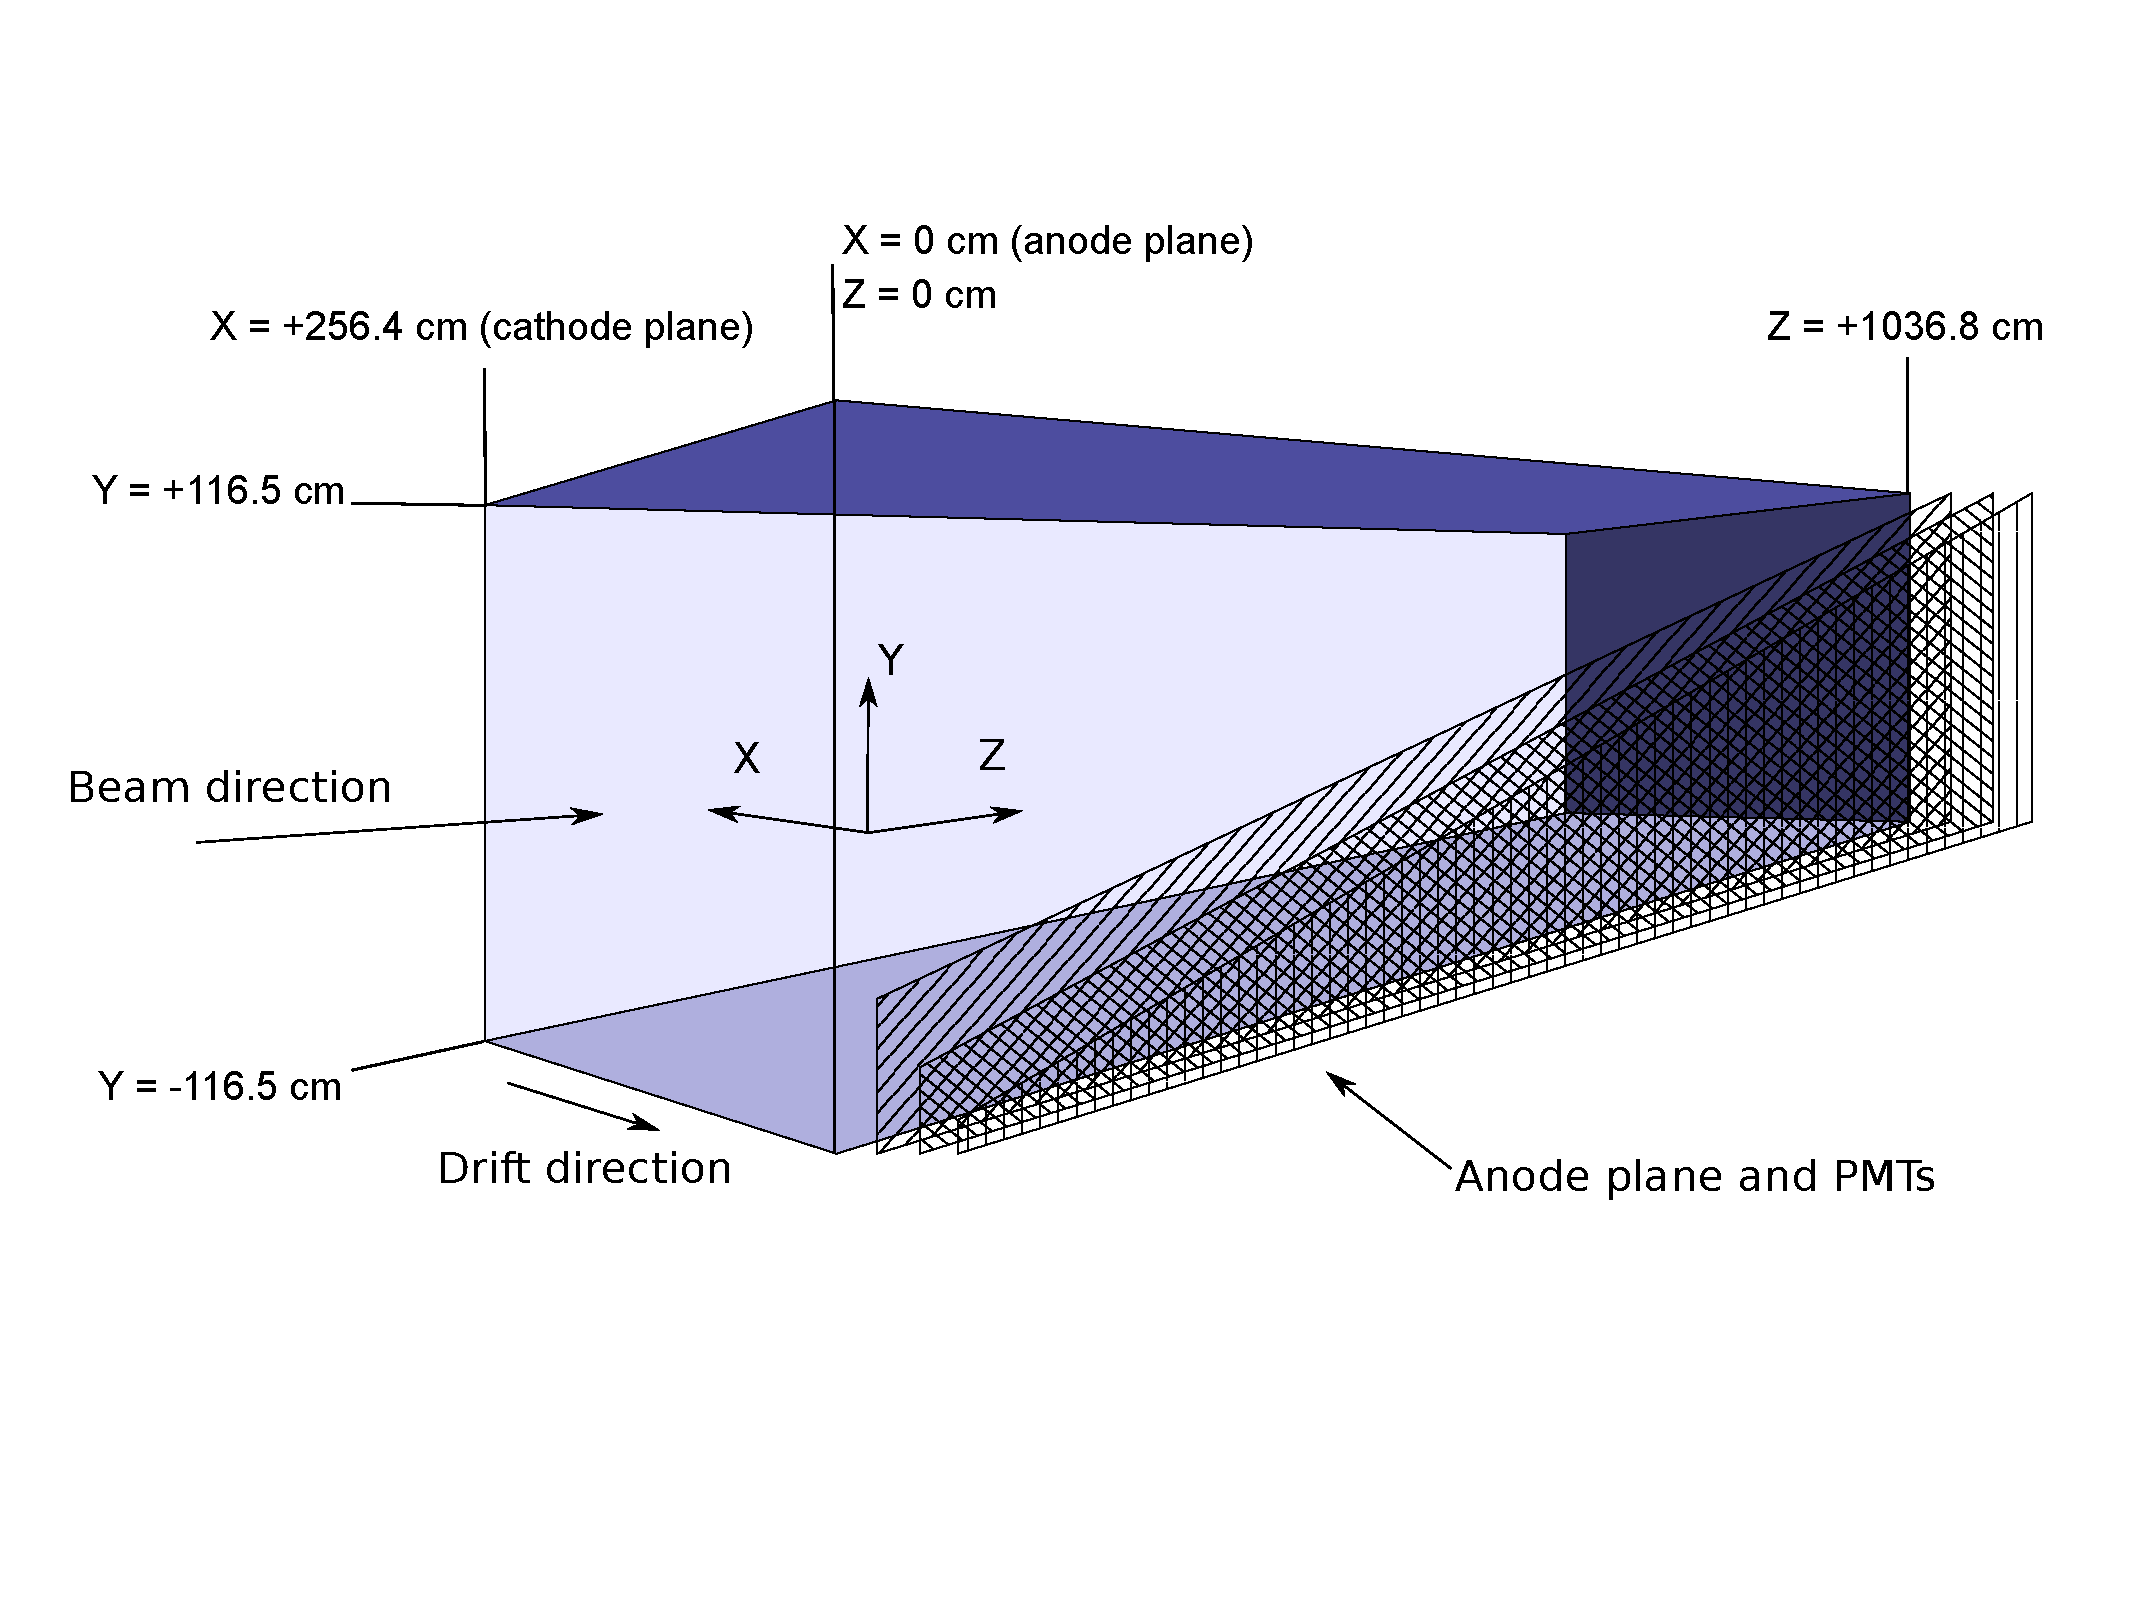
\includegraphics[width=.90\textwidth]{images/MicroBooNE/tpc_coordinates}
\caption[MicroBooNE TPC Coordinate System]{Drawing of the MicroBooNE's \acrshort{tpc}. The \acrshort{tpc} is placed with its longest side in the beam direction. The anode-plane on which wires where signals are formed is on the right-hand side, as seen from the beam. The cathode, where the drift high voltage is applied, is on the left.}
\label{fig:tpc_coordinates}
\end{figure}
The 8256 stainless steel sense wires forming the three anode planes have a plane-to-plane spacing of 3 mm, and the wires on each plane are separated with a 3 mm wire pitch. The wires are connected to application-specific integrated circuits (ASICs) which operate at a liquid argon temperature of 87 K. 
While crossing the first two wire planes, consisting of 2400 wires at angles $\pm$60 degrees relative to the vertical, the electrons induce a signal on them. Subsequently, the electrons are collected by the third plane, made of 3456 vertically-oriented wires.
The electric field is created by a series of 64 2.54-cm diameter stainless steel pipes shaped into a rectangular loop, forming the field cage. The negatively charged cathode is held at a high voltage (operating voltage is 70 kV), and this voltage is incrementally stepped down across the field cage tubes with a voltage divider chain, with an equivalent resistance of 250 M$\Omega$ between each tube. The distance from centre-to-centre of adjacent field cage loops is 4 cm. This creates a uniform electric field within the \acrshort{lartpc}.





\subsection{Charge Signal}
\label{sec:signal_formation}

\begin{figure}[t]
\centering
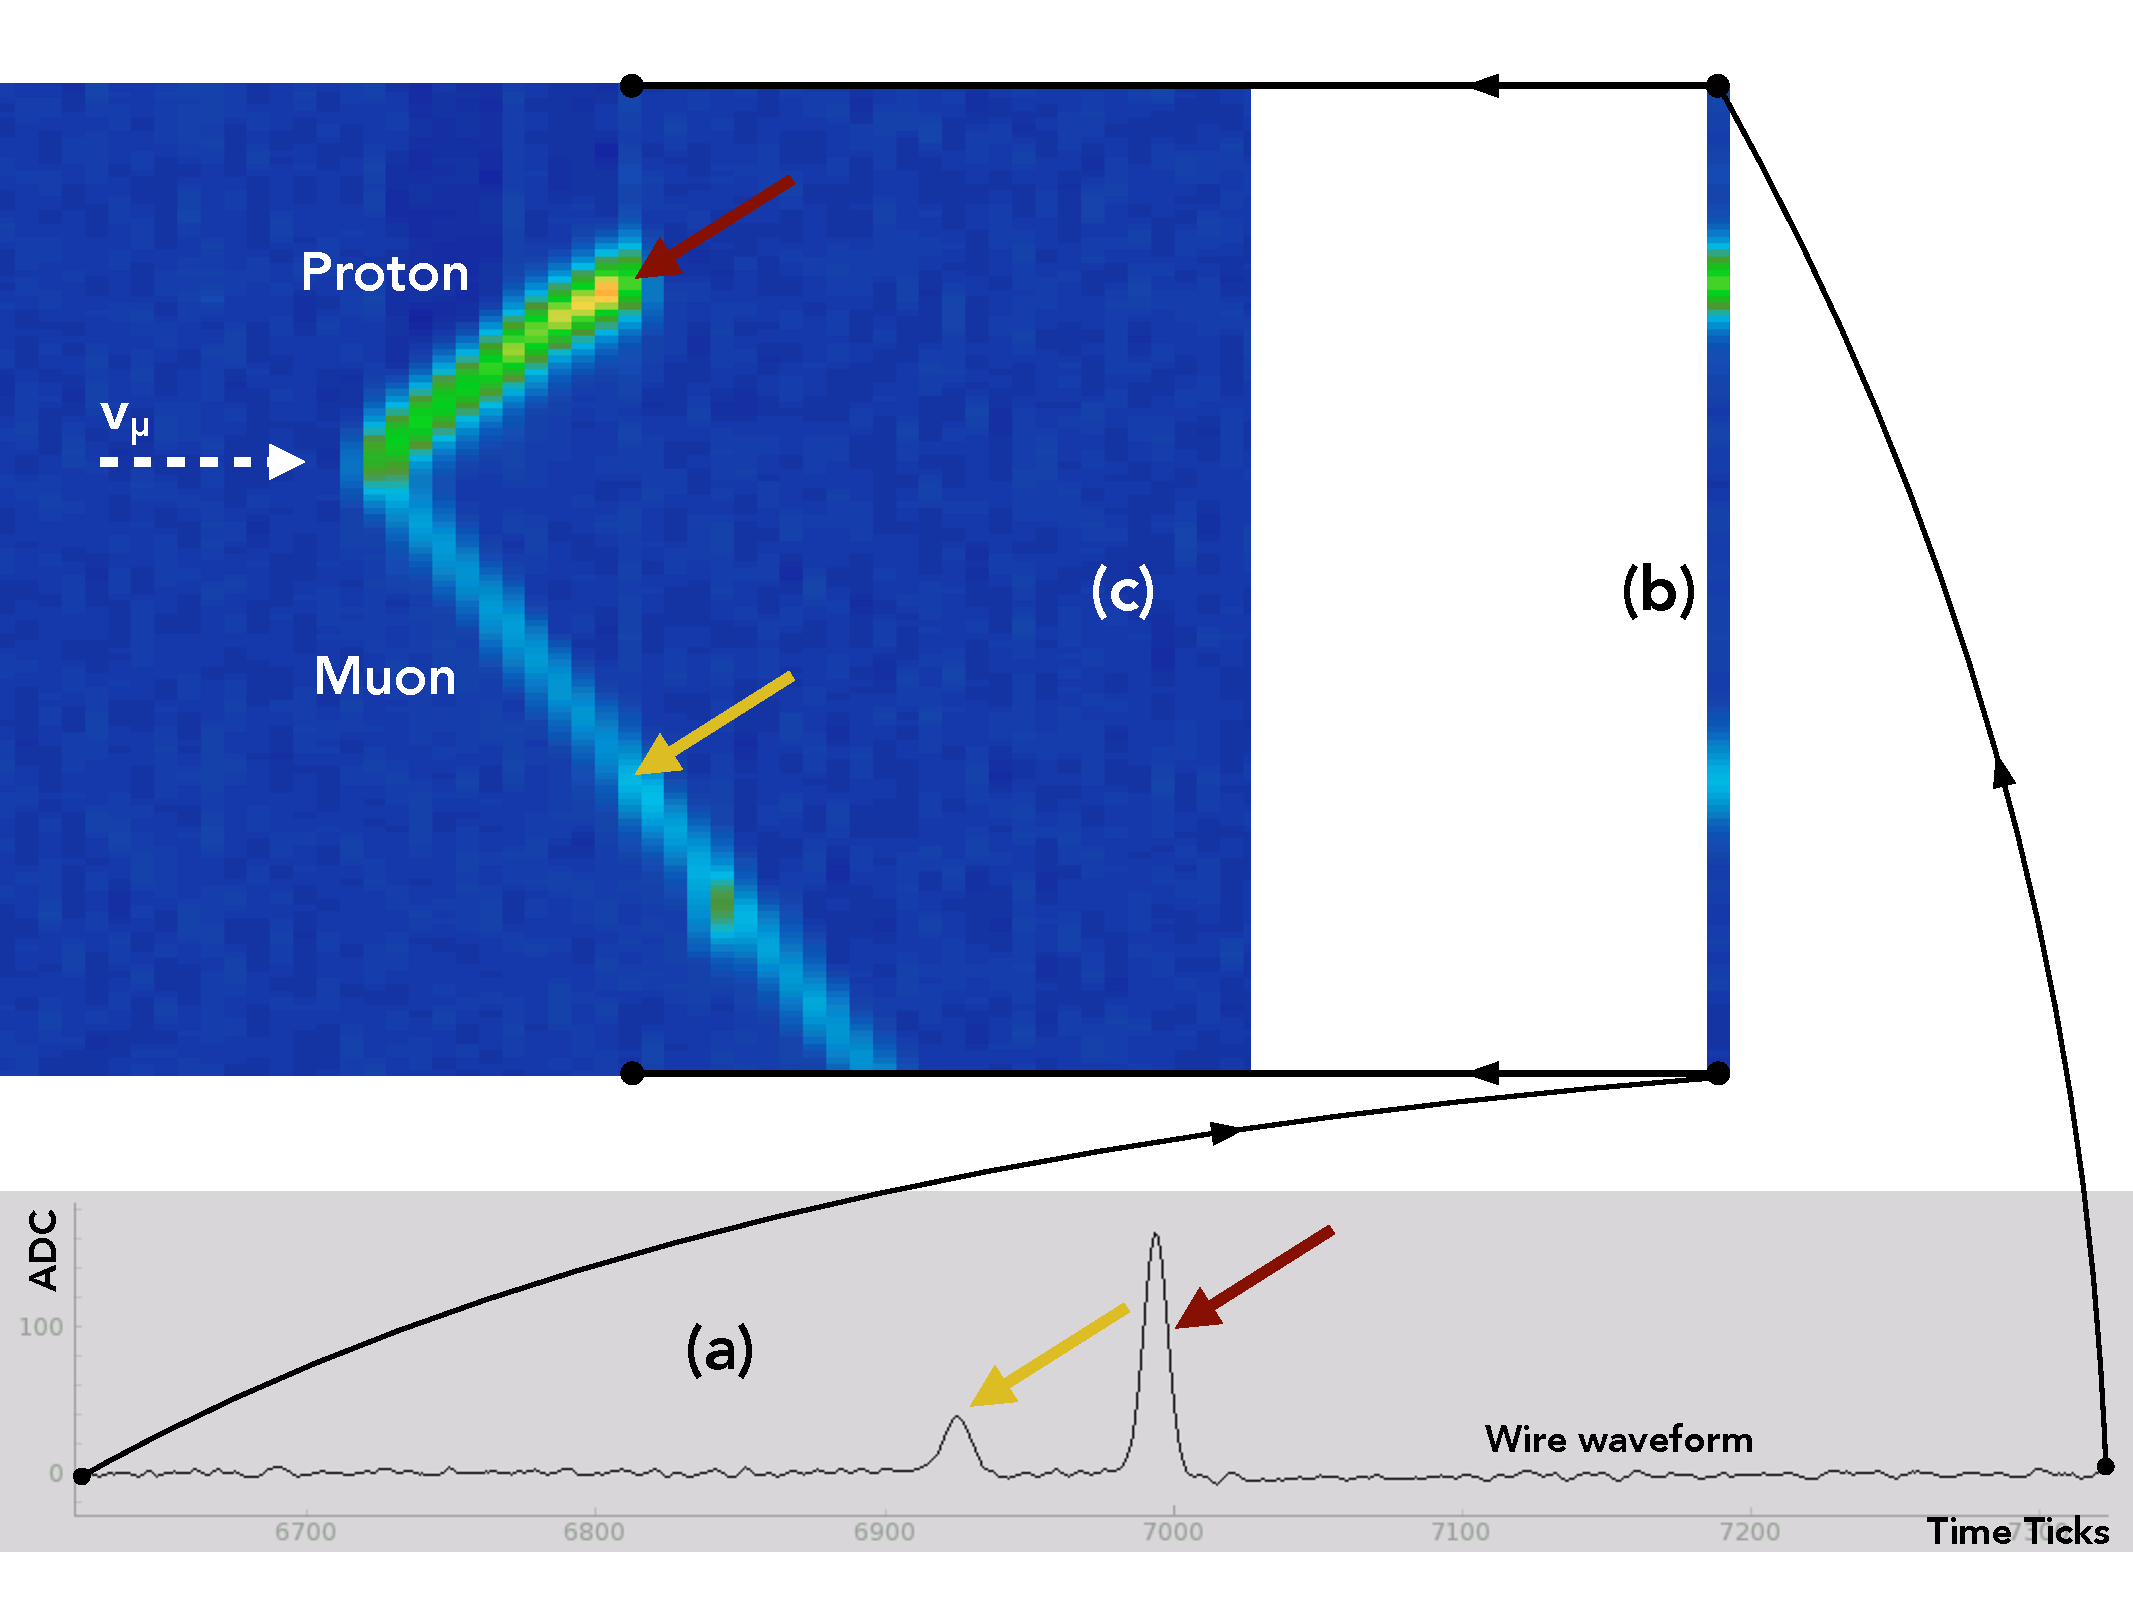
\includegraphics[width=.80\textwidth]{images/MicroBooNE/evd_from_wf}
\caption[MicroBooNE Event Display from Raw Waveform]{Figure (a) shows a waveform from a collection plane wire (after noise filtering~\cite{noise_paper}). Figures (b) and (c) shows how the MicroBooNE event display is constructed, by displaying waveforms from each wire one next to the other. The display shows a candidate interaction vertex from a $\nu_\mu$ \acrshort{cc} interaction, where the final state proton and muon are visible.}
\label{fig:evd_from_wf}
\end{figure}

\begin{figure}[]
\centering
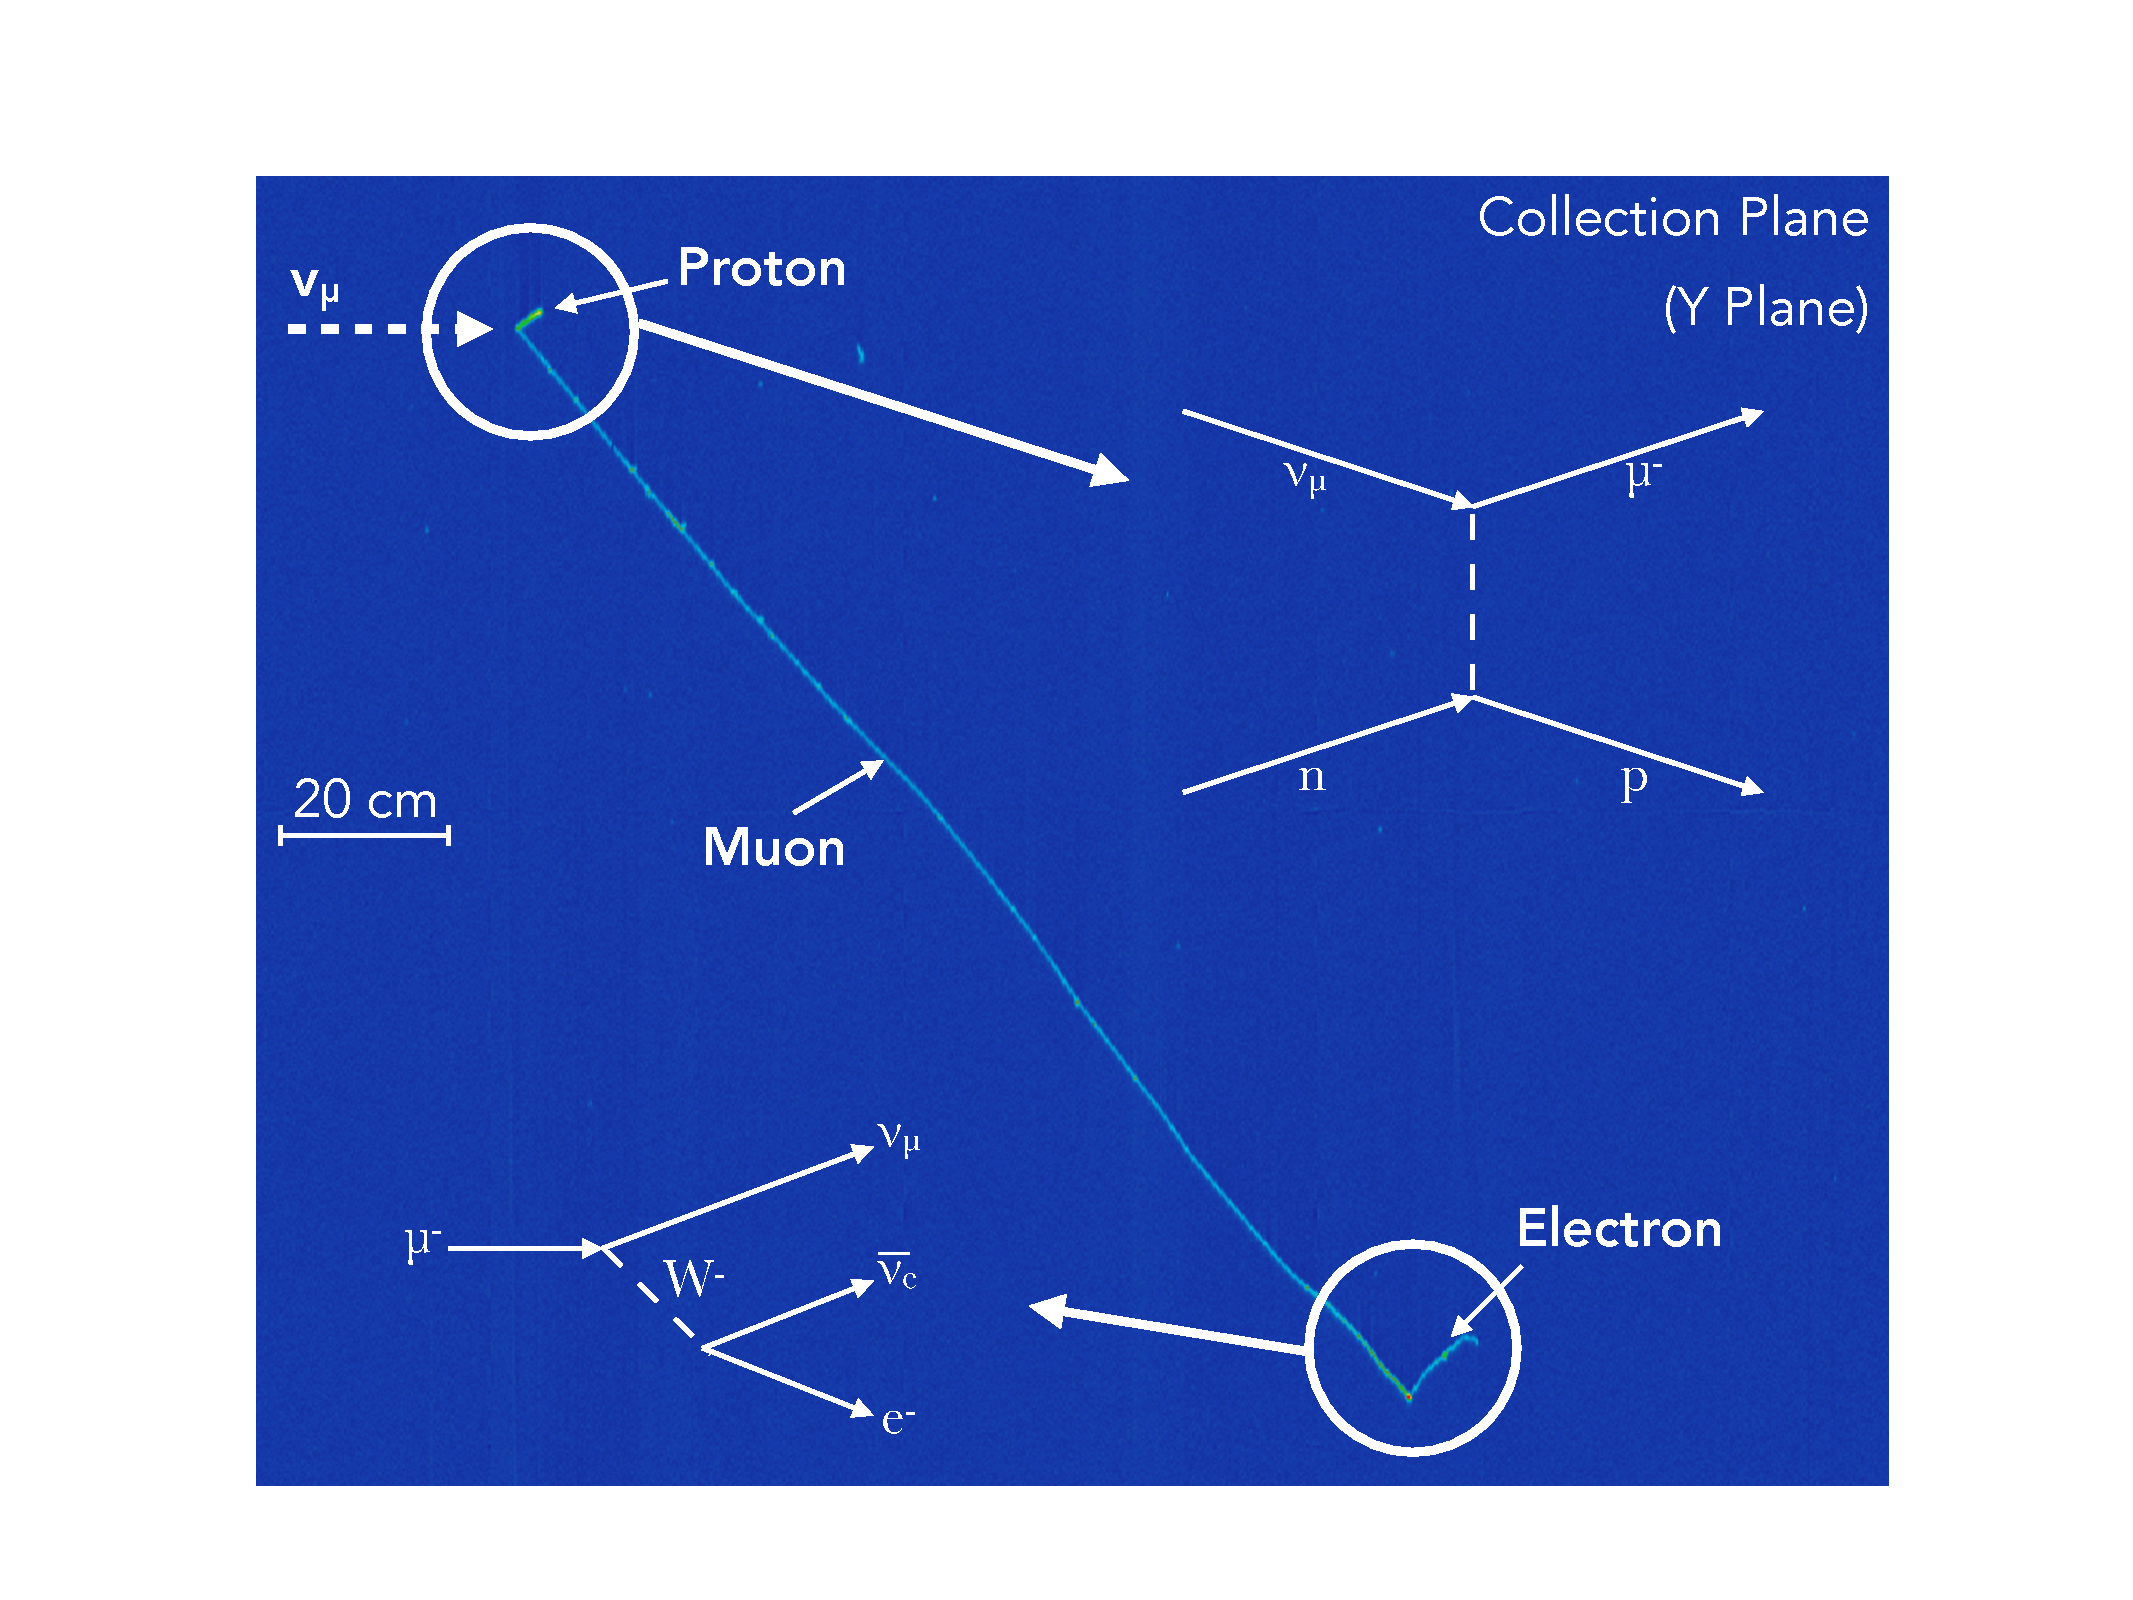
\includegraphics[width=1.0\textwidth]{images/MicroBooNE/evd_2}
\caption[MicroBooNE Event Display with Neutrino Candidate]{Event display showing raw data from a small region of the \acrshort{tpc} volume from the collection plane. The display shows a candidate $\nu_\mu$ \acrshort{cc} interactions, where the final state proton and muon are visible. The $x$ axis shows the collection plane wires (increasing wire-number from left to right) and the $y$ axis shows the drift-coordinate (increasing drift-time moving upwards). The scale bar applies to both the horizontal and vertical coordinates. The colour map shows the amount of collected charge on each wire per time tick. In this display the muon candidate is spatially contained in the detector and it decays. The Michel electron coming from the decay is also visible.}
\label{fig:evd}
\end{figure}

Ionisation electrons produced in the \acrshort{tpc} are detected as induced currents caused by their passage through sense-wires placed on the anode-plane. The same ionisation electrons will produce a signal on wires on all three planes since bias voltages are applied to ensure full transparency of the first two induction planes. As they pass by the first two wire-planes, electrons induce a bipolar signal. The signature on wires on the final plane, on which electrons are collected, is unipolar. Starting with a waveform from a single wire (Figure~\ref{fig:evd_from_wf}, step (a)), it is possible to visualise particles trajectories by displaying such waveform next to the waveforms from all the other wires, as done in steps (b) and (c) of Figure~\ref{fig:evd_from_wf}. This figure only shows part of the detector, where a $\nu_\mu$ \acrshort{cc} candidate vertex was identified. Figure~\ref{fig:evd} shows the complete candidate event, with the final state muon coming o a stop and decaying. In this figure, moving from the left to right, all the waveforms from the collection plane wires are displayed. For a single wire, the $y$ axis shows the recorded waveform in drift-time coordinate. Particle trajectory points visible in the lower part of the image are closer to the anode plane, as it took less time for the electrons originated in those points to drift and be collected by the collection plane wires. The $y$ axis in this figure can then be seen as the drift direction in the detector, while the $x$ axis shows the direction along the neutrino beam, as collection plane wires are displaced perpendicularly to this direction. In summary, Figure~\ref{fig:evd} shows a bird-eye view of particles interacting in the MicroBooNE detector.


\subsection{Light Collection System}
\label{sec:pmt}

Liquid argon is a bright scintillator, and sampling the light produced from interactions in the argon can bring powerful capabilities and information to complement the charge information. Scintillation light is produced by the formation and eventual radiative decay of excited argon dimers (or excimers) and is emitted in an isotropic distribution~\cite{doke, kubota}. Liquid argon produces a large amount of light per unit energy deposited (about 24,000 photons per MeV at 500 V/cm drift field) and is transparent to its own scintillation. The scintillation light has one prompt and one slow component with decay times of about 6 ns and 1.6 $\mu$s, respectively. 
Both components consist of photons with a wavelength of 128 nm (VUV). An example of raw waveform recorded by a single \acrshort{pmt} in MicroBooNE from a candidate neutrino interaction is shown in Figure~\ref{fig:raw_wf}, where both the fast and slow components are visible.

\begin{figure}[]
\centering
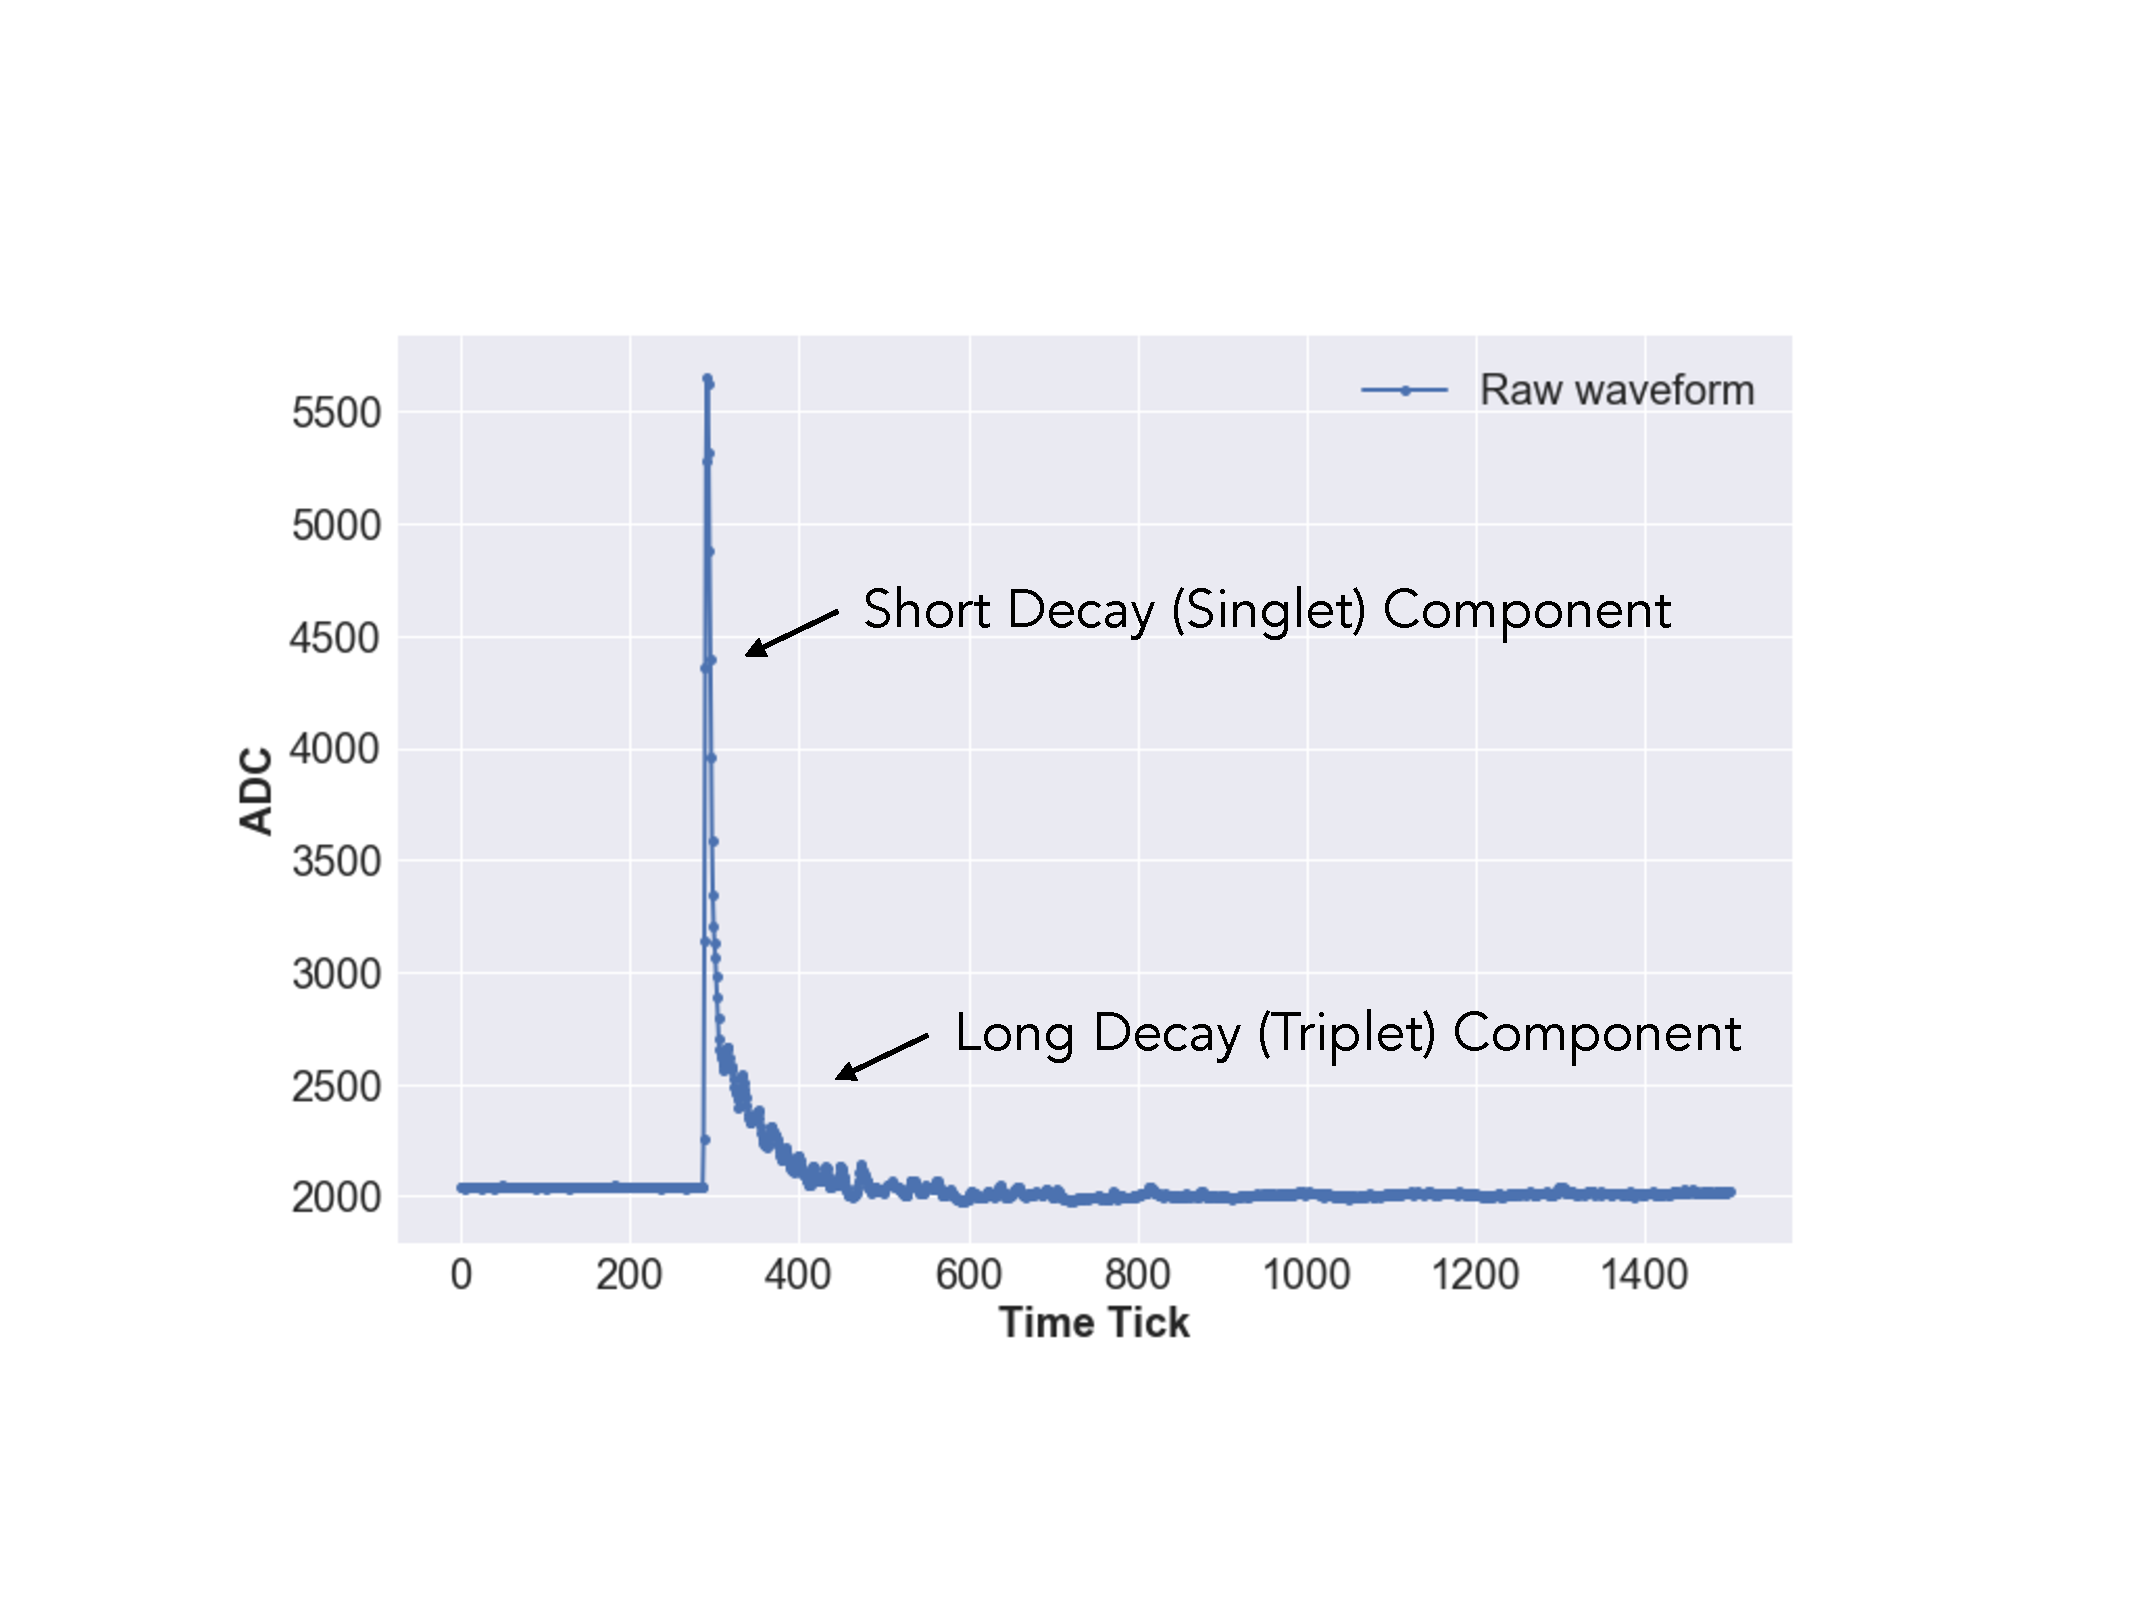
\includegraphics[width=.70\textwidth]{images/MicroBooNE/raw_wf}
\caption[MicroBooNE Optical Waveform]{A waveform from a MicroBooNE optical detector from the \acrshort{pmt} shaper (see Section~\ref{sec:readout_data_format}). One time-tick corresponds to 15.6 ns.}
\label{fig:raw_wf}
\end{figure}

Scintillation light is an important ingredient to the ultimate 3D reconstruction of particle interactions within a \acrshort{lartpc}. While the wire signals alone suffice to reconstruct 3D interactions, the absolute timing of an interaction (referred to as $t_0$) is unknown so there is ambiguity in the drift direction. However, measuring the scintillation light allows to clarify this ambiguity to high precision. In fact, the time scale of the production and propagation of the light (nanoseconds) is orders of magnitude faster than the ionisation electrons drift (milliseconds). Furthermore, the scintillation light from interactions is relatively localised, and therefore combining the measured \acrshort{pmt} signals with the physical position of the signal allows to match individual flashes of light with different interactions, which may have different interaction times $t_0$. The description of this flash-to-track matching is provided in Section~\ref{sec:flashmatch}. This is important to help tagging and rejecting cosmogenic backgrounds which may occur outside of the expected beam neutrino arrival times.

\begin{figure}[]
\centering
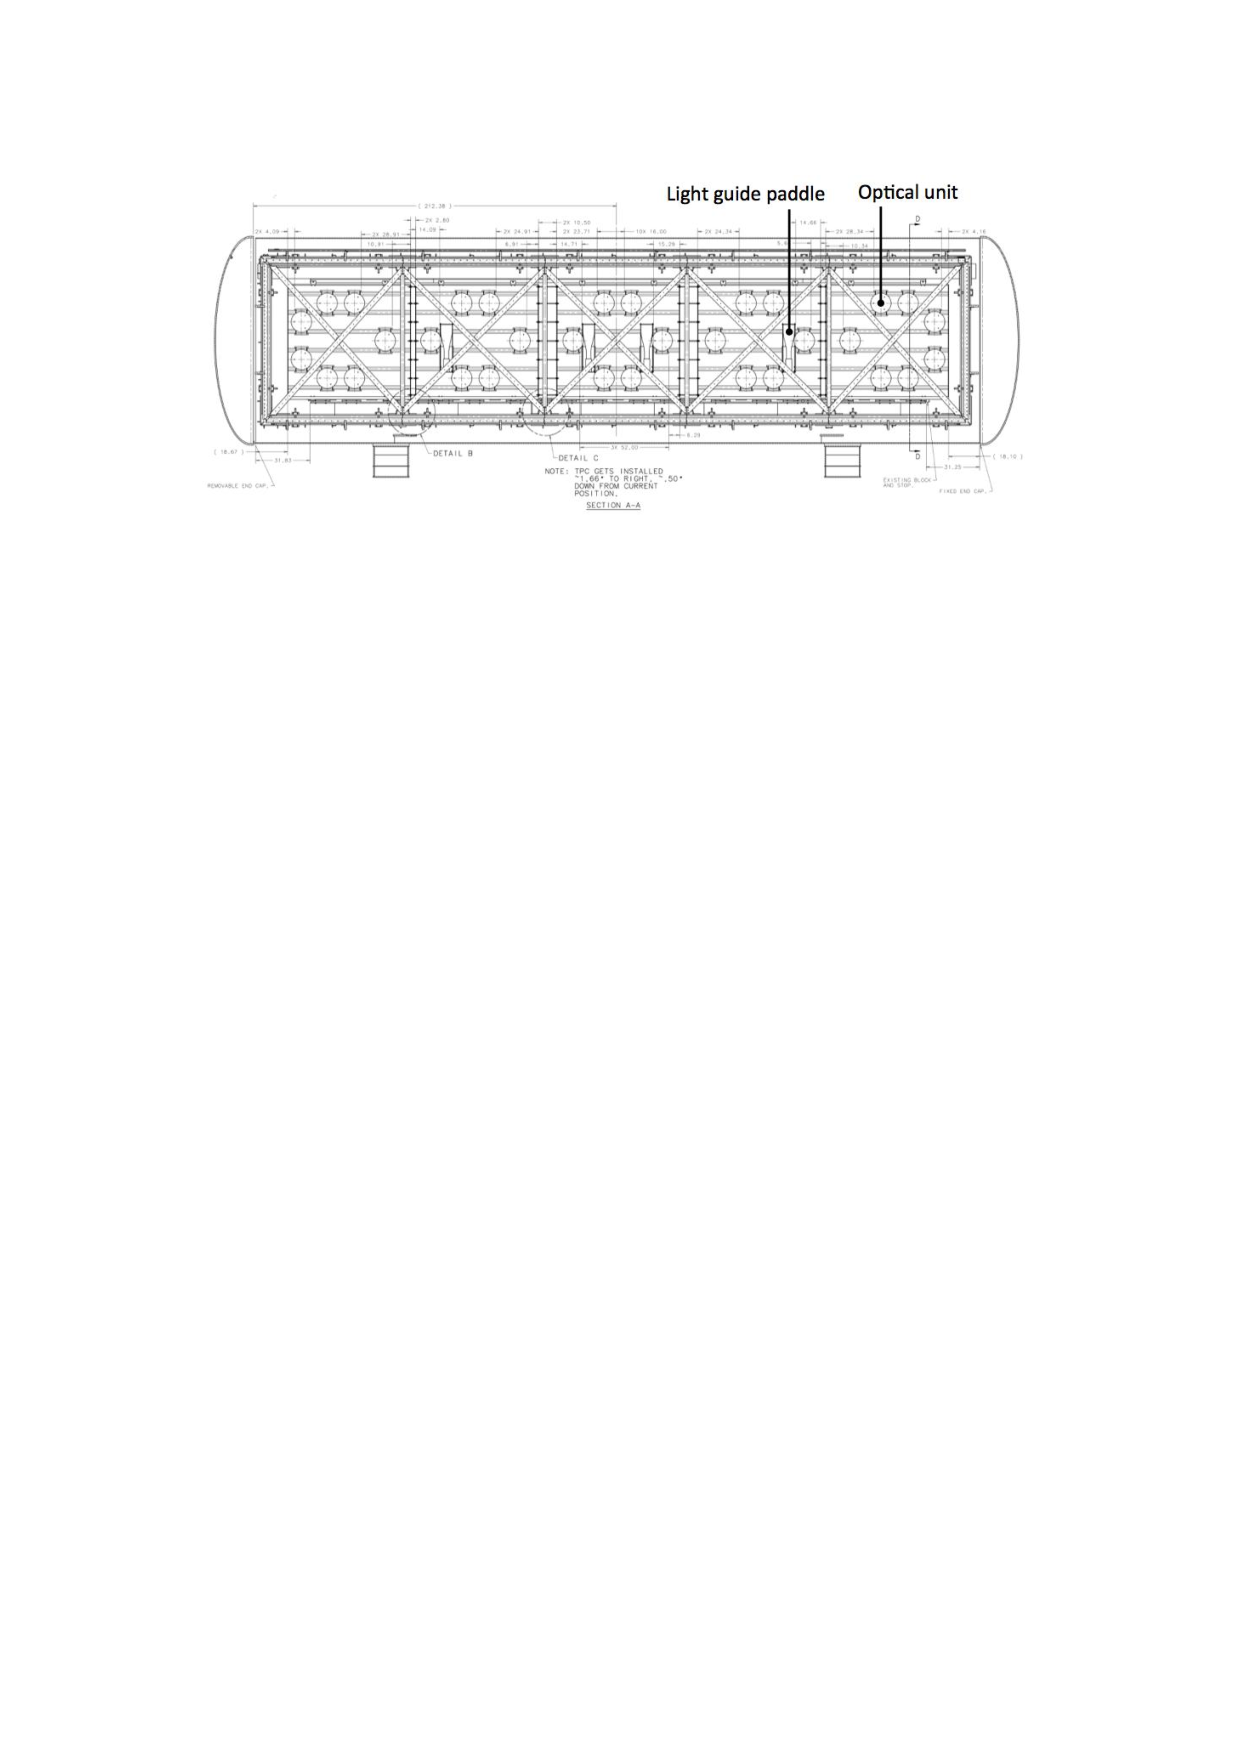
\includegraphics[width=.80\textwidth]{images/MicroBooNE/pmt_map}
\caption[MicroBooNE Light Collection System]{The MicroBooNE light collection system consists of a primary system of 32 optical units and a secondary optical system of four light guide paddles \cite{ub_paddle}. These are mounted behind the anode wire planes such that the view is not obscured by structural cross bars of the \acrshort{lartpc}. Image credit: \cite{det}.}
\label{fig:pmt_map}
\end{figure}

The light collection system in MicroBooNE consists of 32 8-inch-diameter Hamamatsu R5912-02mod cryogenic \acrshort{pmt}s. These \acrshort{pmt}s are mounted in a plane behind the three sense-wire planes. The physical location of these \acrshort{pmt}s is shown in Figure~\ref{fig:pmt_map}. These 32 \acrshort{pmt}s provide 0.9\% photocathode coverage. As shown in Figure~\ref{fig:pmt_pics}, in front of each \acrshort{pmt} an acrylic plate is mounted, coated with \acrfull{tpb}, an organic fluor which serves as a wavelength-shifting material. \acrshort{tpb} absorbs the VUV scintillation light photons and re-emits it at visible wavelengths detectable by the \acrshort{pmt}s, peaked at 425 nm.

%\begin{figure}[]
%\centering
%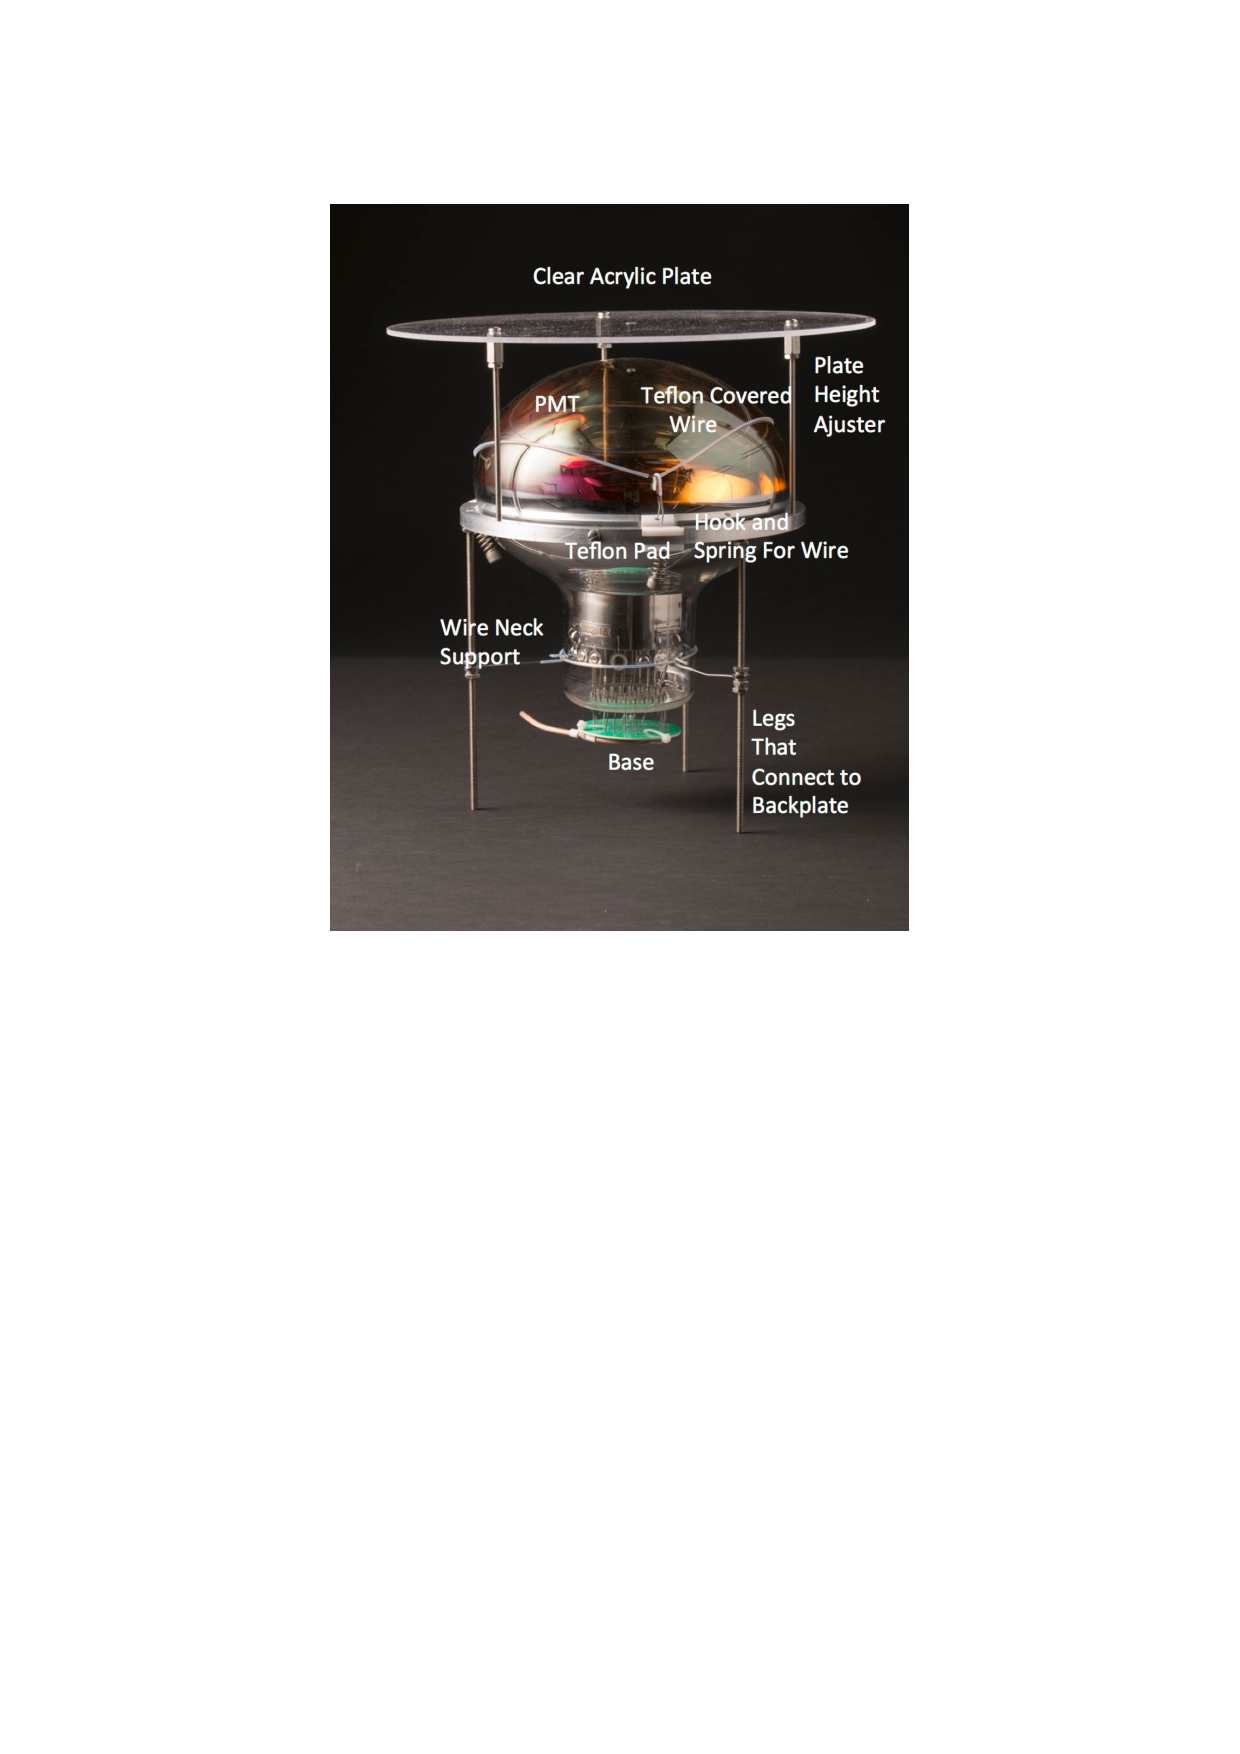
\includegraphics[width=.40\textwidth]{images/MicroBooNE/pmt_ub}
%\caption[MicroBooNE Optical Unit]{The MicroBooNE optical unit mount internal to the shield, with components labeled. Image credit: \cite{det}.}
%\label{fig:pmt_ub}
%\end{figure}

\begin{figure}[]
\centering
\subfloat[][]
   {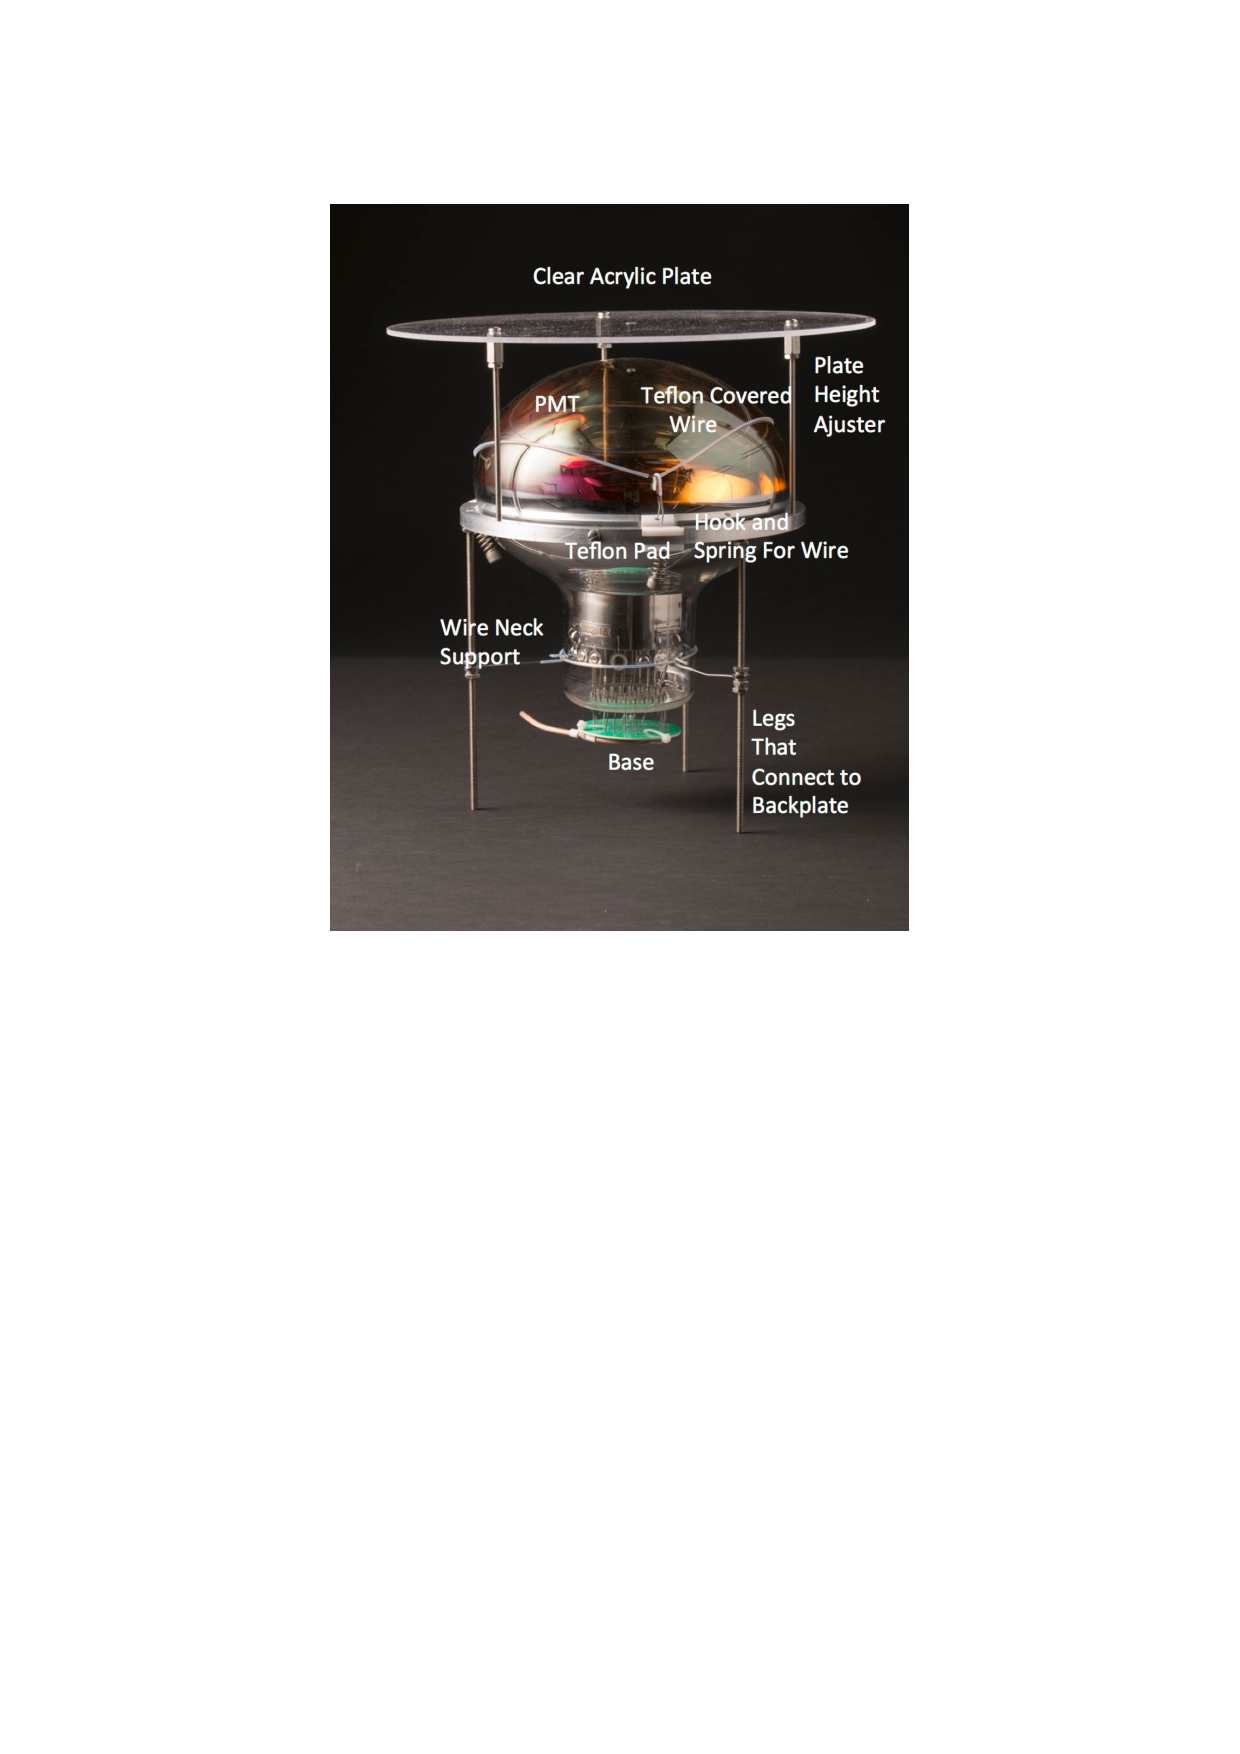
\includegraphics[height=.43\textwidth]{images/MicroBooNE/pmt_ub}
   \label{fig:pmt_ub}} 
\subfloat[][]
   {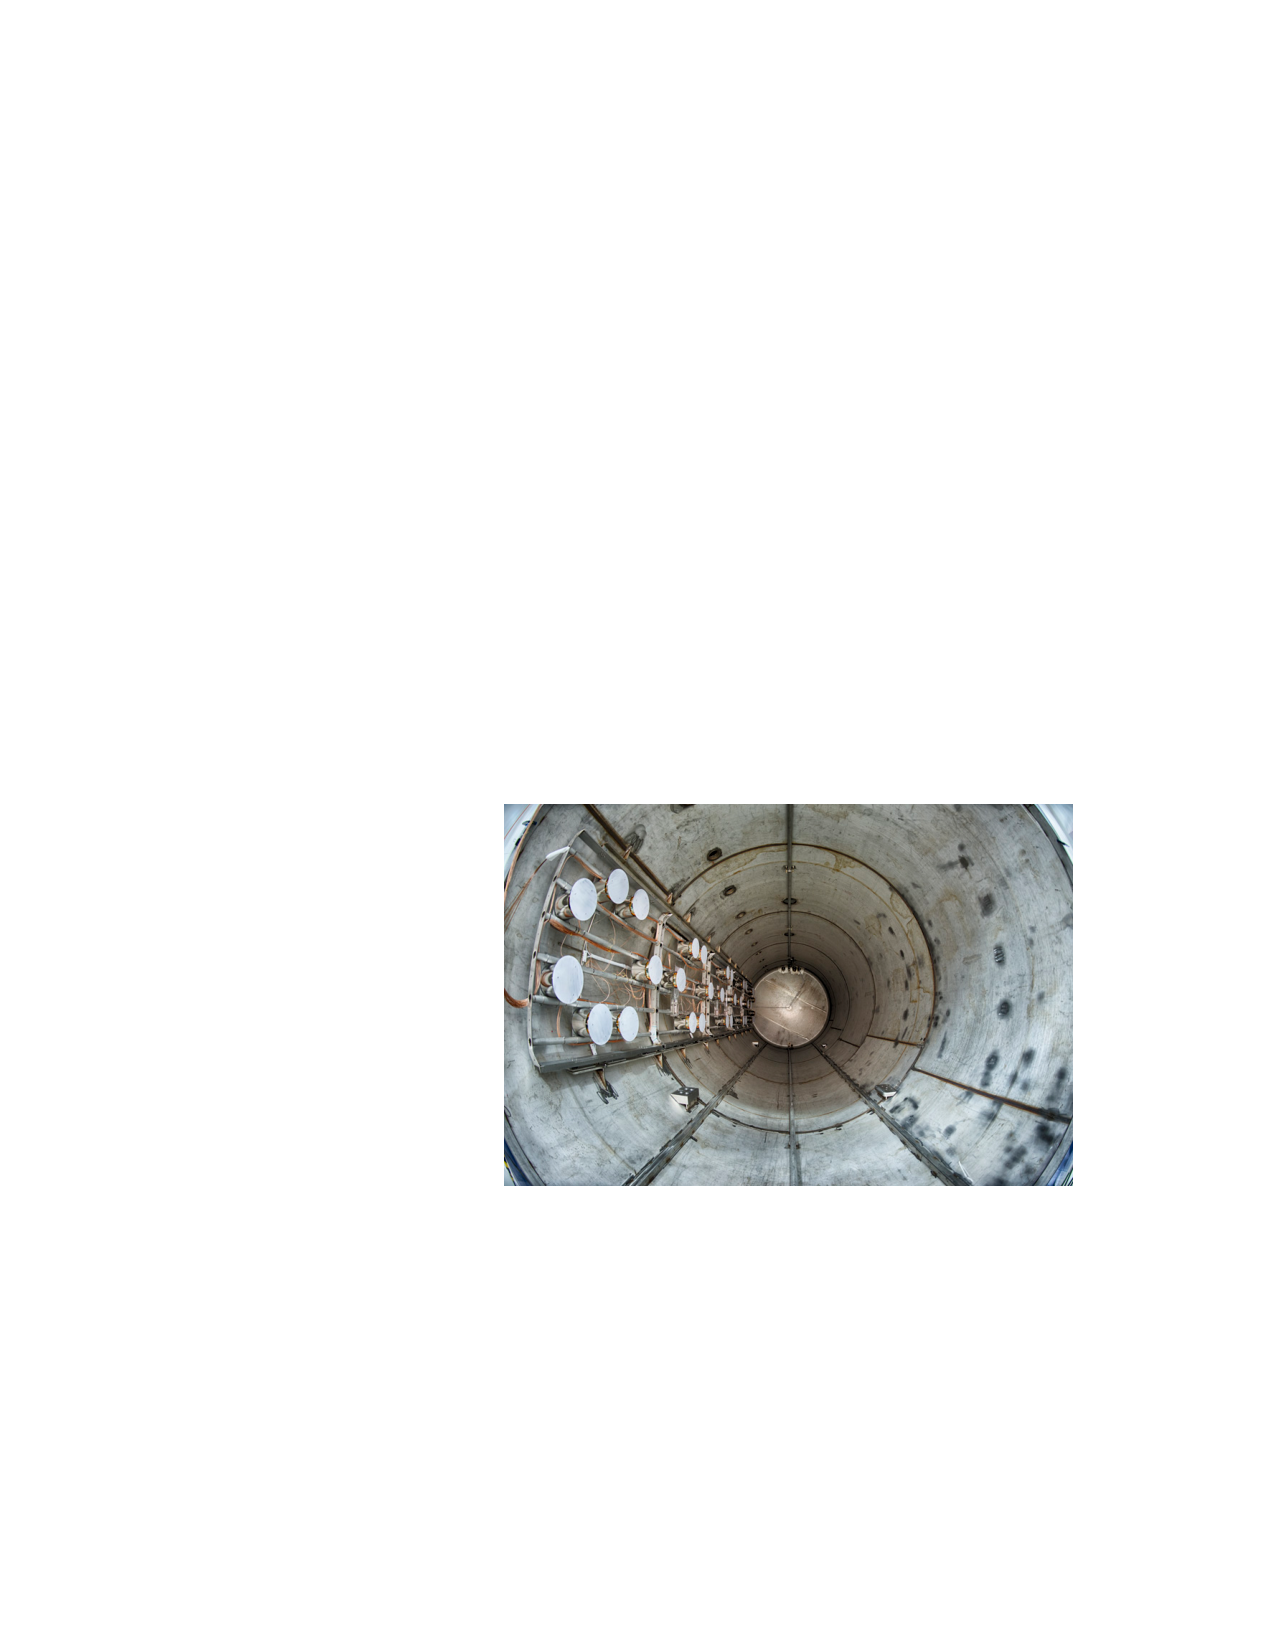
\includegraphics[height=.43\textwidth]{images/MicroBooNE/pmt_pic_cryo}
   \label{fig:pmt_pic_cryo}}
\caption[MicroBooNE Optical Unit]{The MicroBooNE optical unit mount internal to the shield, with components labeled~\protect\subref{fig:pmt_ub}. Photo credit: \cite{det}. \acrshort{pmt}s mounted on the frame inside the MicroBooNE cryostat ~\protect\subref{fig:pmt_pic_cryo}. Photo credit: Reidar Hahn, Fermilab Visual Media Services.}
\label{fig:pmt_pics}
\end{figure}




\section{Triggers and Data Streams}
\label{sec:trigger}

Every event in MicroBooNE starts with a hardware trigger. The Fermilab accelerator division sends signals to MicroBooNE every time there is a neutrino beam spill. This trigger, called the ``\acrshort{bnb}'' trigger, causes a window to open the \acrshort{pmt} readout that lasts for 23.4 $\mu$s, and a window in the \acrshort{tpc} readout that lasts 4.8 ms. The beam trigger efficiency is 99.8\%~\cite{CaratelliThesis}. The data sample originating from the trigger is here called ``beam-on'' data sample.

The majority of the spills do not produce a neutrino interaction in the detector.  Indeed, simulations show that approximately only 1 in 600 beam spills produces a neutrino interaction in the detector. In order to reduce the amount of recorded data, not every spill is saved. A software trigger looks at light activity on the \acrshort{pmt}s in time-coincidence with the 1.6 $\mu$s beam spill reaching the detector. 
This activity may be caused by a neutrino interaction, coincident \acrshort{cr} activity, or some other coincident sources.
The software trigger reduces the data rate by a factor of 20 \cite{CaratelliThesis}. The signal efficiency loss through the trigger condition is negligibly small. Additionally, the trigger cut is superseded by a higher optical light deposition cut, later in the analysis. 

An additional trigger used in this work is the so-called ``EXT'' trigger, that mimics a \acrshort{bnb} trigger in the absence of neutrino beam. This trigger allows to record \acrshort{cr} data in order to measure the cosmogenic background that will affect the analysis. The data sample collected with this trigger is here called ``beam-off'' data sample.

In order to reduce the data volume to apply \acrshort{tpc} reconstruction algorithms to, an optical pre-filter is also run. This filter checks for optical activity within the time window of the beam and requires a minimum threshold of 20 \acrfull{pe} in the beam time window (a study on the impact of a \acrshort{pe} threshold on the analysis is described in Section~\ref{sec:beam_spill}).

The MicroBooNE simulation (described in Section~\ref{sec:simulation}), only includes simulation of events that contain neutrino interactions and does not contain events with only \acrshort{cr}s. In order to be compared to the beam-on data sample, events from the beam-off data stream are added to the simulation, normalising by the number of hardware triggers.
The event distributions presented in this thesis will either show simulation compared to beam-on minus beam-off data, or simulation plus beam-off data compared to beam-on data.




\section[Readout and Data Format]{Readout Electronics and Data Format}
\label{sec:readout_data_format}

MicroBooNE's readout electronics are responsible for forming, digitising, and recording signals associated with the \acrshort{tpc} and \acrshort{pmt} systems. 

The MicroBooNE \acrshort{tpc} electronics system is separated in ``cold'' electronics, submerged in liquid argon, and ``warm'' electronics, located outside of the cryostat. The cold electronics is responsible for amplifying and shaping signals produced on the sense wires. Performing these operations in a cold environment and in close proximity to the wires allows MicroBooNE to obtain a high signal-to-noise ratio, essential to obtain accurate particle identification with low detection thresholds. The warm electronics is responsible for digitising signals, compressing and formatting the data before it is sent to the data acquisition system.

The analogue signals from the 8256 sense wires in the \acrshort{tpc} pass through \acrfull{cmos} analogue front end ASICs which operate on cold motherboards at liquid argon temperatures~\cite{det}. The signals are then shaped and amplified by cold intermediate amplifiers before passing through a warm feed-through. The signals are received by custom-designed \acrshort{lartpc} readout modules, which digitise and process them. The \acrshort{tpc} wire signals are digitised at 16 MHz and then down-sampled in the digitisation process to 2 MHz (500 ns time-ticks). The \acrshort{tpc} system reads out three 1.6 ms frames of wire signal data associated with one event. This time is chosen based on how long it takes for ionisation electrons from the cathode side of the \acrshort{tpc} to drift to the anode wires (this time is 1.6 ms with the design drift field of 500 V/cm, but 2.3 ms with the current MicroBooNE drift field of 173 V/cm). One frame before and two frames after the trigger are collected, ensuring enough amount of data to identify a neutrino interaction, as well as all \acrshort{cr} signals that arrive soon enough before or after the neutrino which need to be reconstructed in analyses.

Similarly to the \acrshort{tpc}, the \acrshort{pmt} signals undergo separate shaping with a 60 ns peaking time to allow for digitisation of several samples on the rising edge of a signal for more precise timing reconstruction abilities. The \acrshort{pmt} signals are digitised at 64 MHz (15.625 ns time-ticks) and are then split into high-gain and low-gain channels which carry 18\% and 1.8\% of the total signal amplitude, respectively, to extend the dynamic range of the \acrfull{adc}.
The \acrshort{pmt} system records data in two different formats: $(i)$ in an unbiased way for a duration of 1500 samples (23.4 $\mu$s) which is opened by the beam-gate signal received on the trigger board. Neutrinos are expected to arrive $\sim$ 4 $\mu$s after this window is opened; $(ii)$ in a discriminated way (called ``cosmic discriminator'') before and after the 23.4 $\mu$s window. This is needed in order to reduce the amount of recorded data. Discriminated waveforms are read out for an interval of 6.4 ms, which well covers the 4.8 ms \acrshort{tpc} readout window: $[-1.6, +3.2]$ ms. The cosmic discriminator only saves waveforms that go above a threshold of 130 \acrshort{adc} ($\sim6.5$ effective \acrshort{pe}), and it only saves 40 samples ($\sim$ 0.6 $\mu$s). A dead-time of 45 samples follows every time a cosmic-discriminated waveform is recorded.











\section{Simulation}
\label{sec:simulation}


Beamline and detector simulations are intended to represent truth level estimations of neutrino production and interaction processes. These estimations serve as a baseline for comparison with collected data, as well as to estimate the backgrounds in the selected data samples. They are referred to as \acrfull{mc} simulations. There are a number of systems to model, and details to account for, to ensure the simulation precisely captures the state of the detector.

The flux of neutrinos at the MicroBooNE detector is simulated using a framework built by the MiniBooNE collaboration \cite{miniboone_flux}.
Neutrino interactions in the MicroBooNE detector are simulated using the \textsc{Genie} event generator \cite{GENIE}, which generates the primary interaction inside the argon nucleus, the production of all final-state particles in the nucleus (hadronisation), and the transport and rescattering of the final-state particles through the nucleus (\acrshort{fsi}).

\begin{figure}[t]
\centering
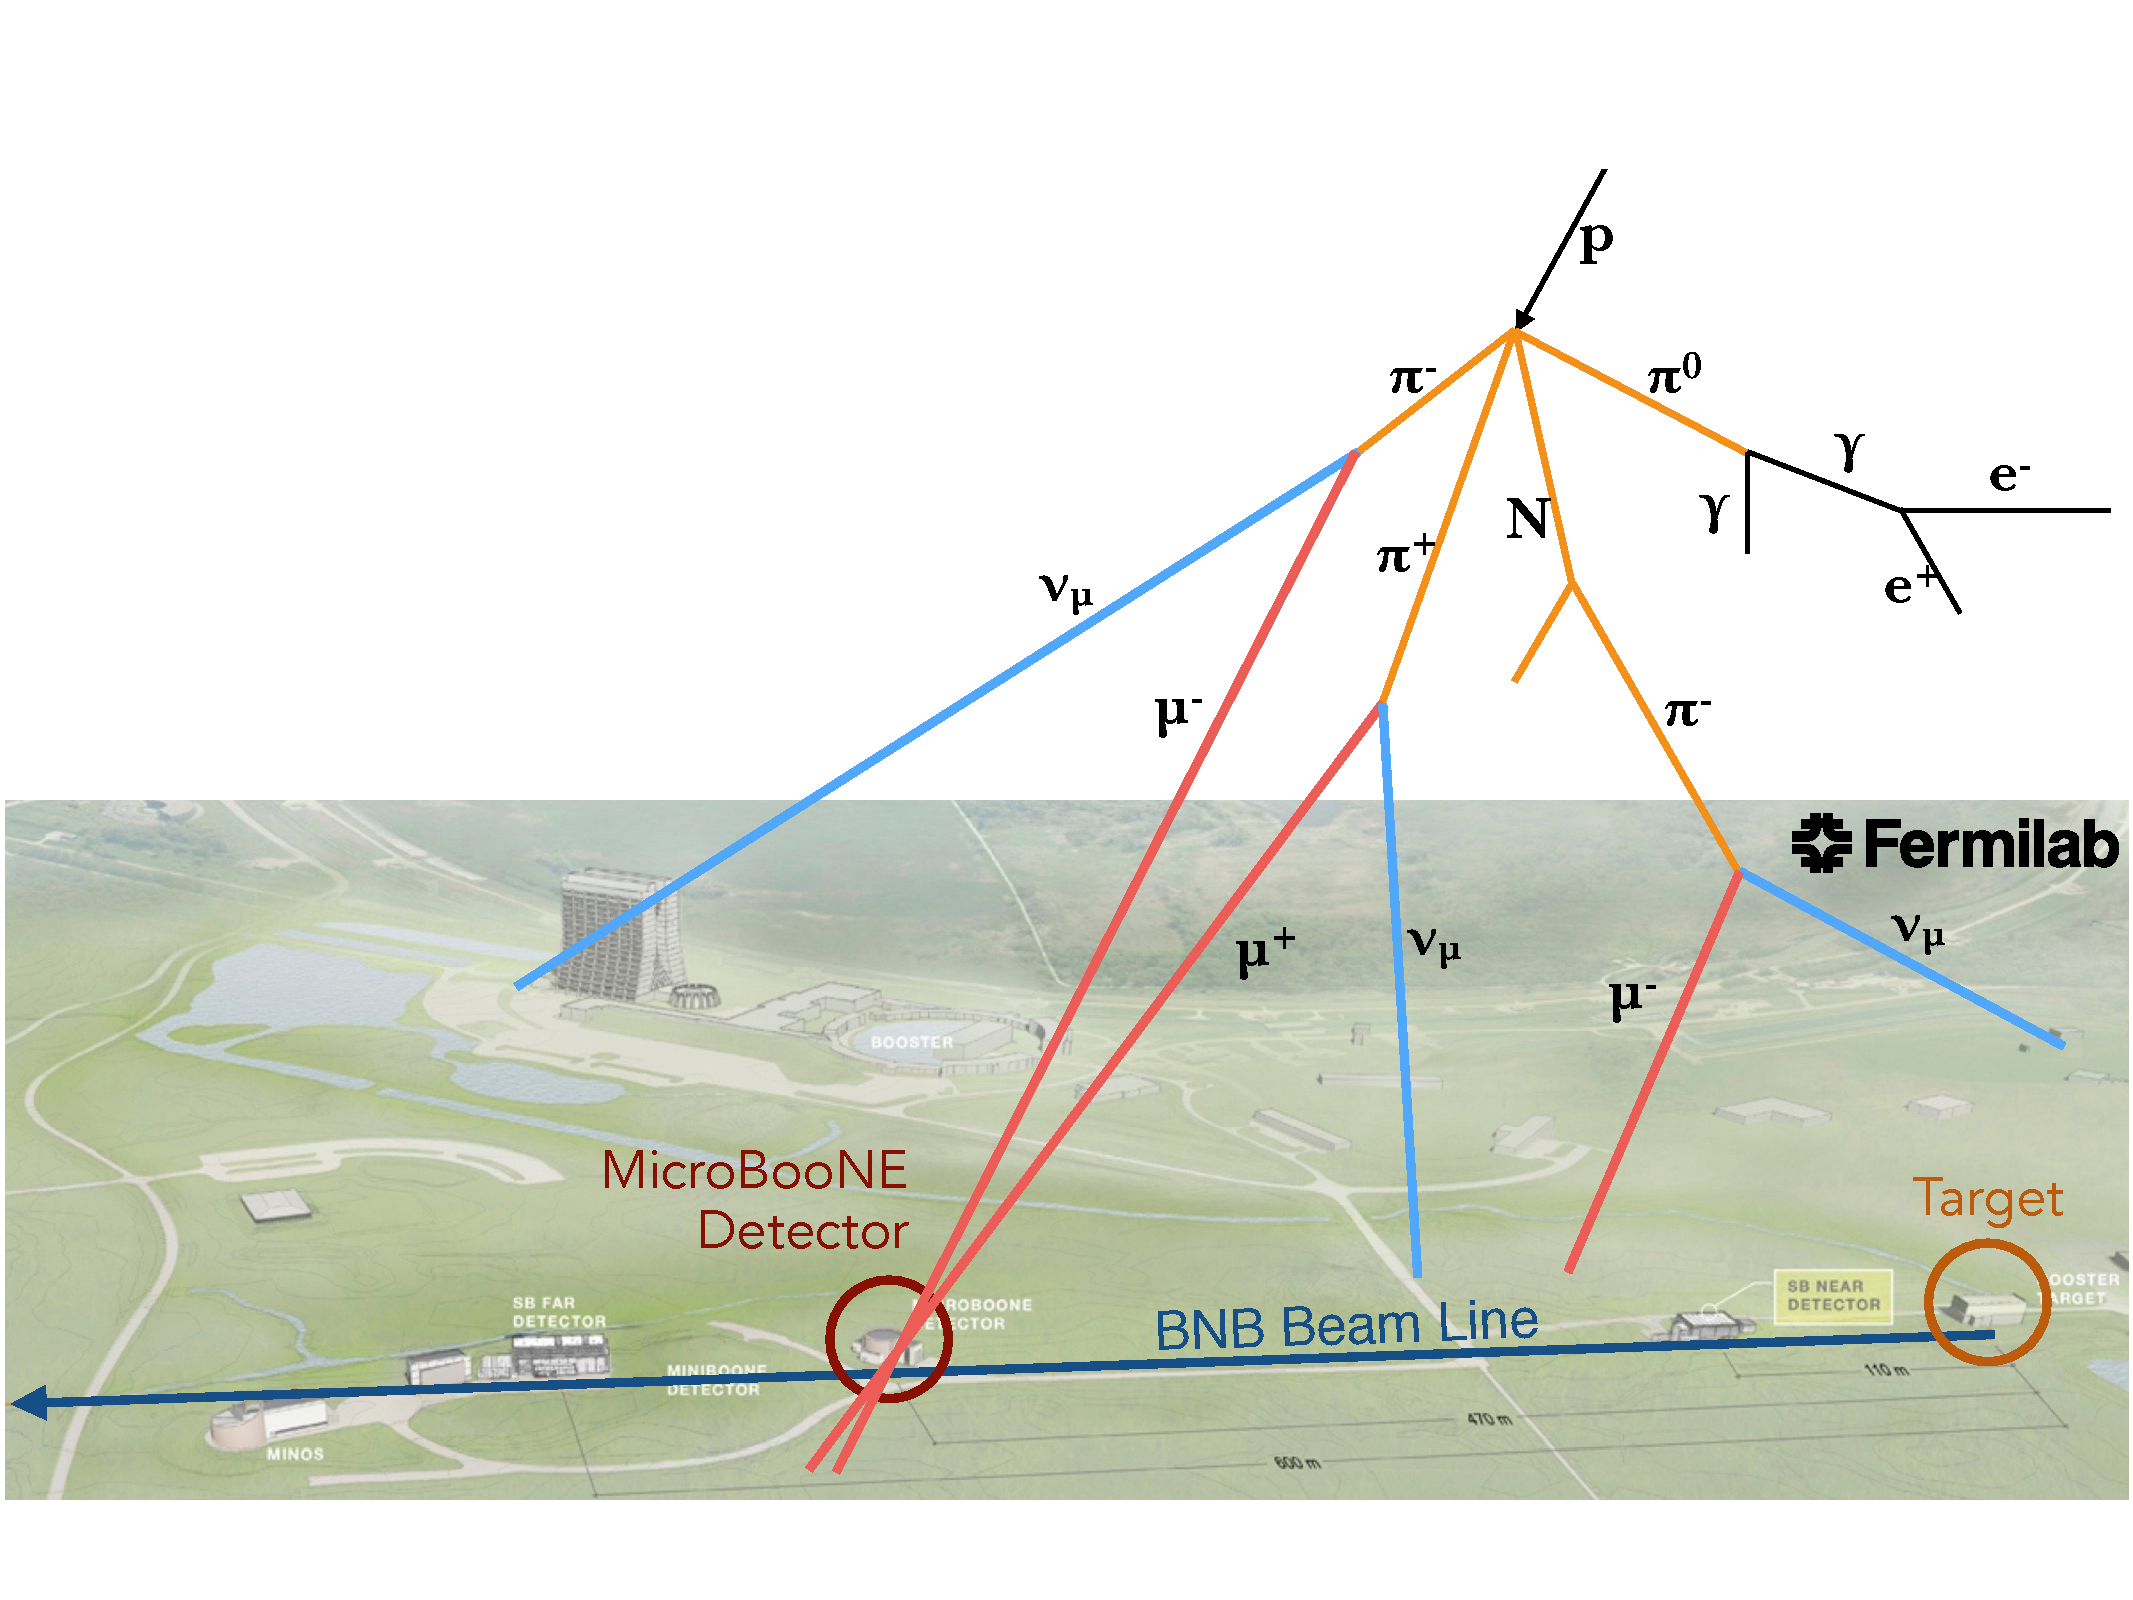
\includegraphics[width=1.0\textwidth]{images/MicroBooNE/sbn_cosmics}
\caption[Aerial View of Fermilab with Cosmic Rays]{Aerial view of Fermilab with the Booster neutrino beamline and the MicroBooNE detector. \acrshort{cr}s are the dominant background for many MicroBooNE data analyses.}
\label{fig:sbn_cosmics}
\end{figure}

Before proceeding with the detector simulation, there is one final step. MicroBooNE is a surface detector and is then subject to a high \acrshort{cr} rate, and many \acrshort{cr} muons cross the detector as shown in Figure~\ref{fig:sbn_cosmics}. The detector is placed in a pit 6 m below the surface with no overburden, and the estimated rate is of 5.5 kHz, which corresponds to an average of 25 \acrshort{cr} muons per recorded event. 
%
\begin{figure}[]
\centering
\subfloat[][]
   {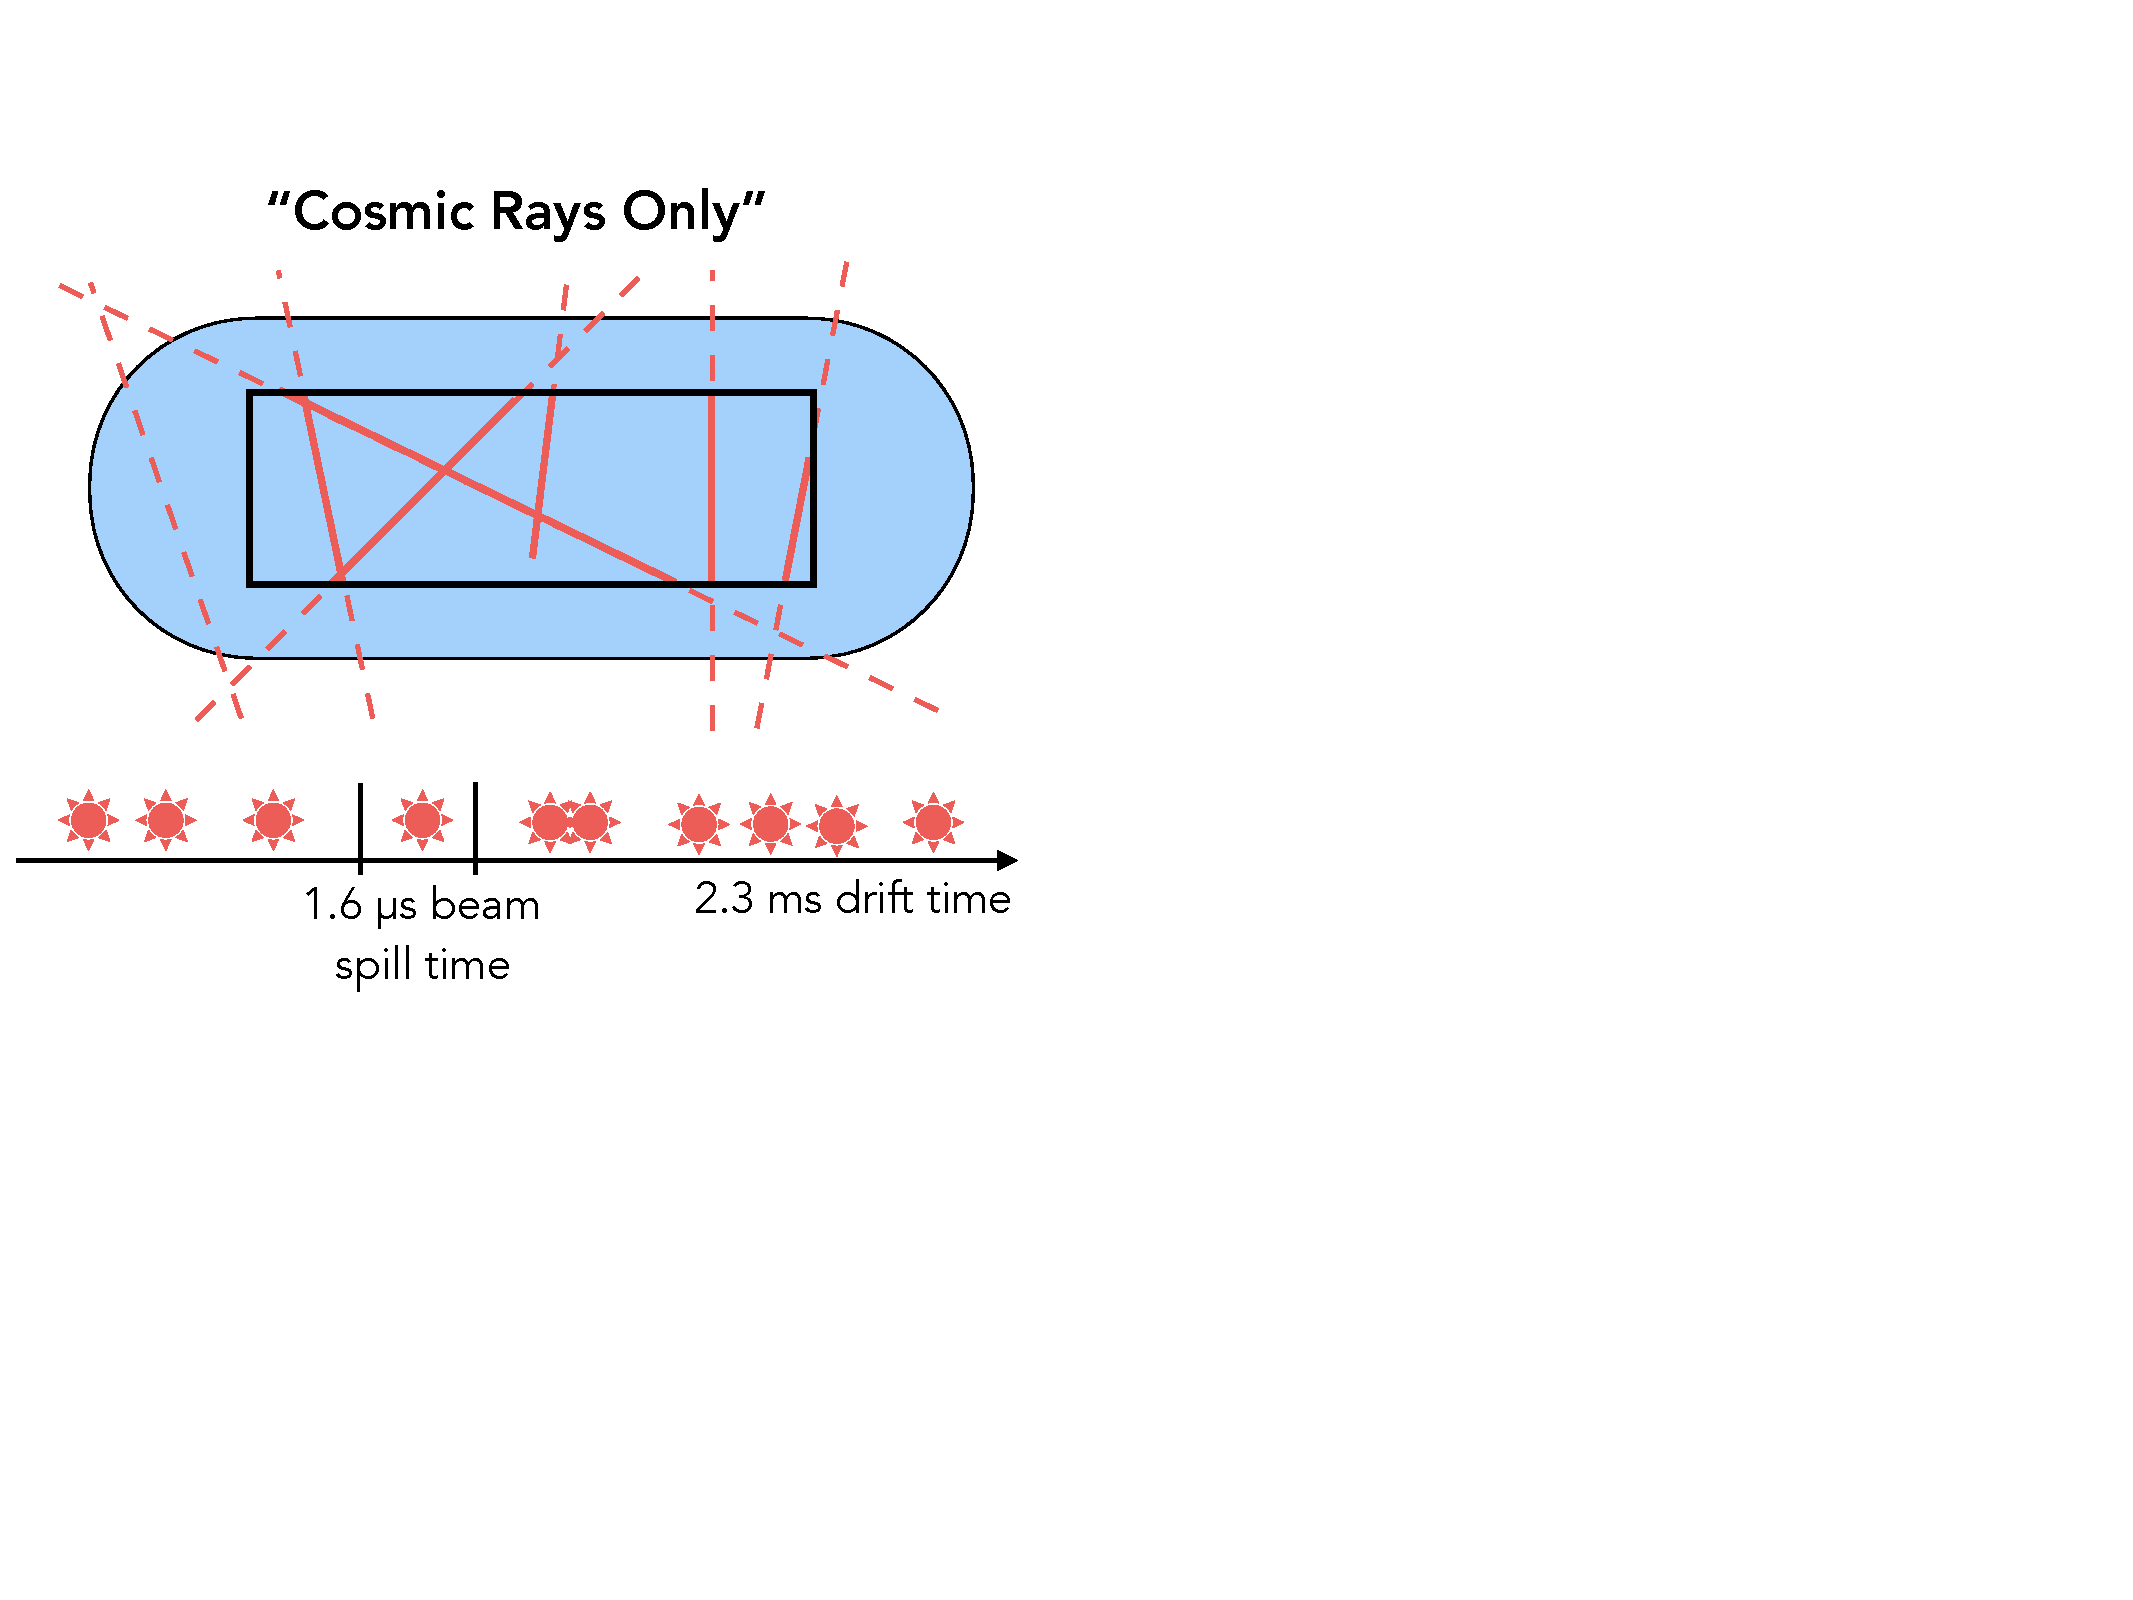
\includegraphics[width=.48\textwidth]{images/MicroBooNE/beam_on_beam_off_a}
   \label{fig:beam_on_beam_off_a}} 
\subfloat[][]
   {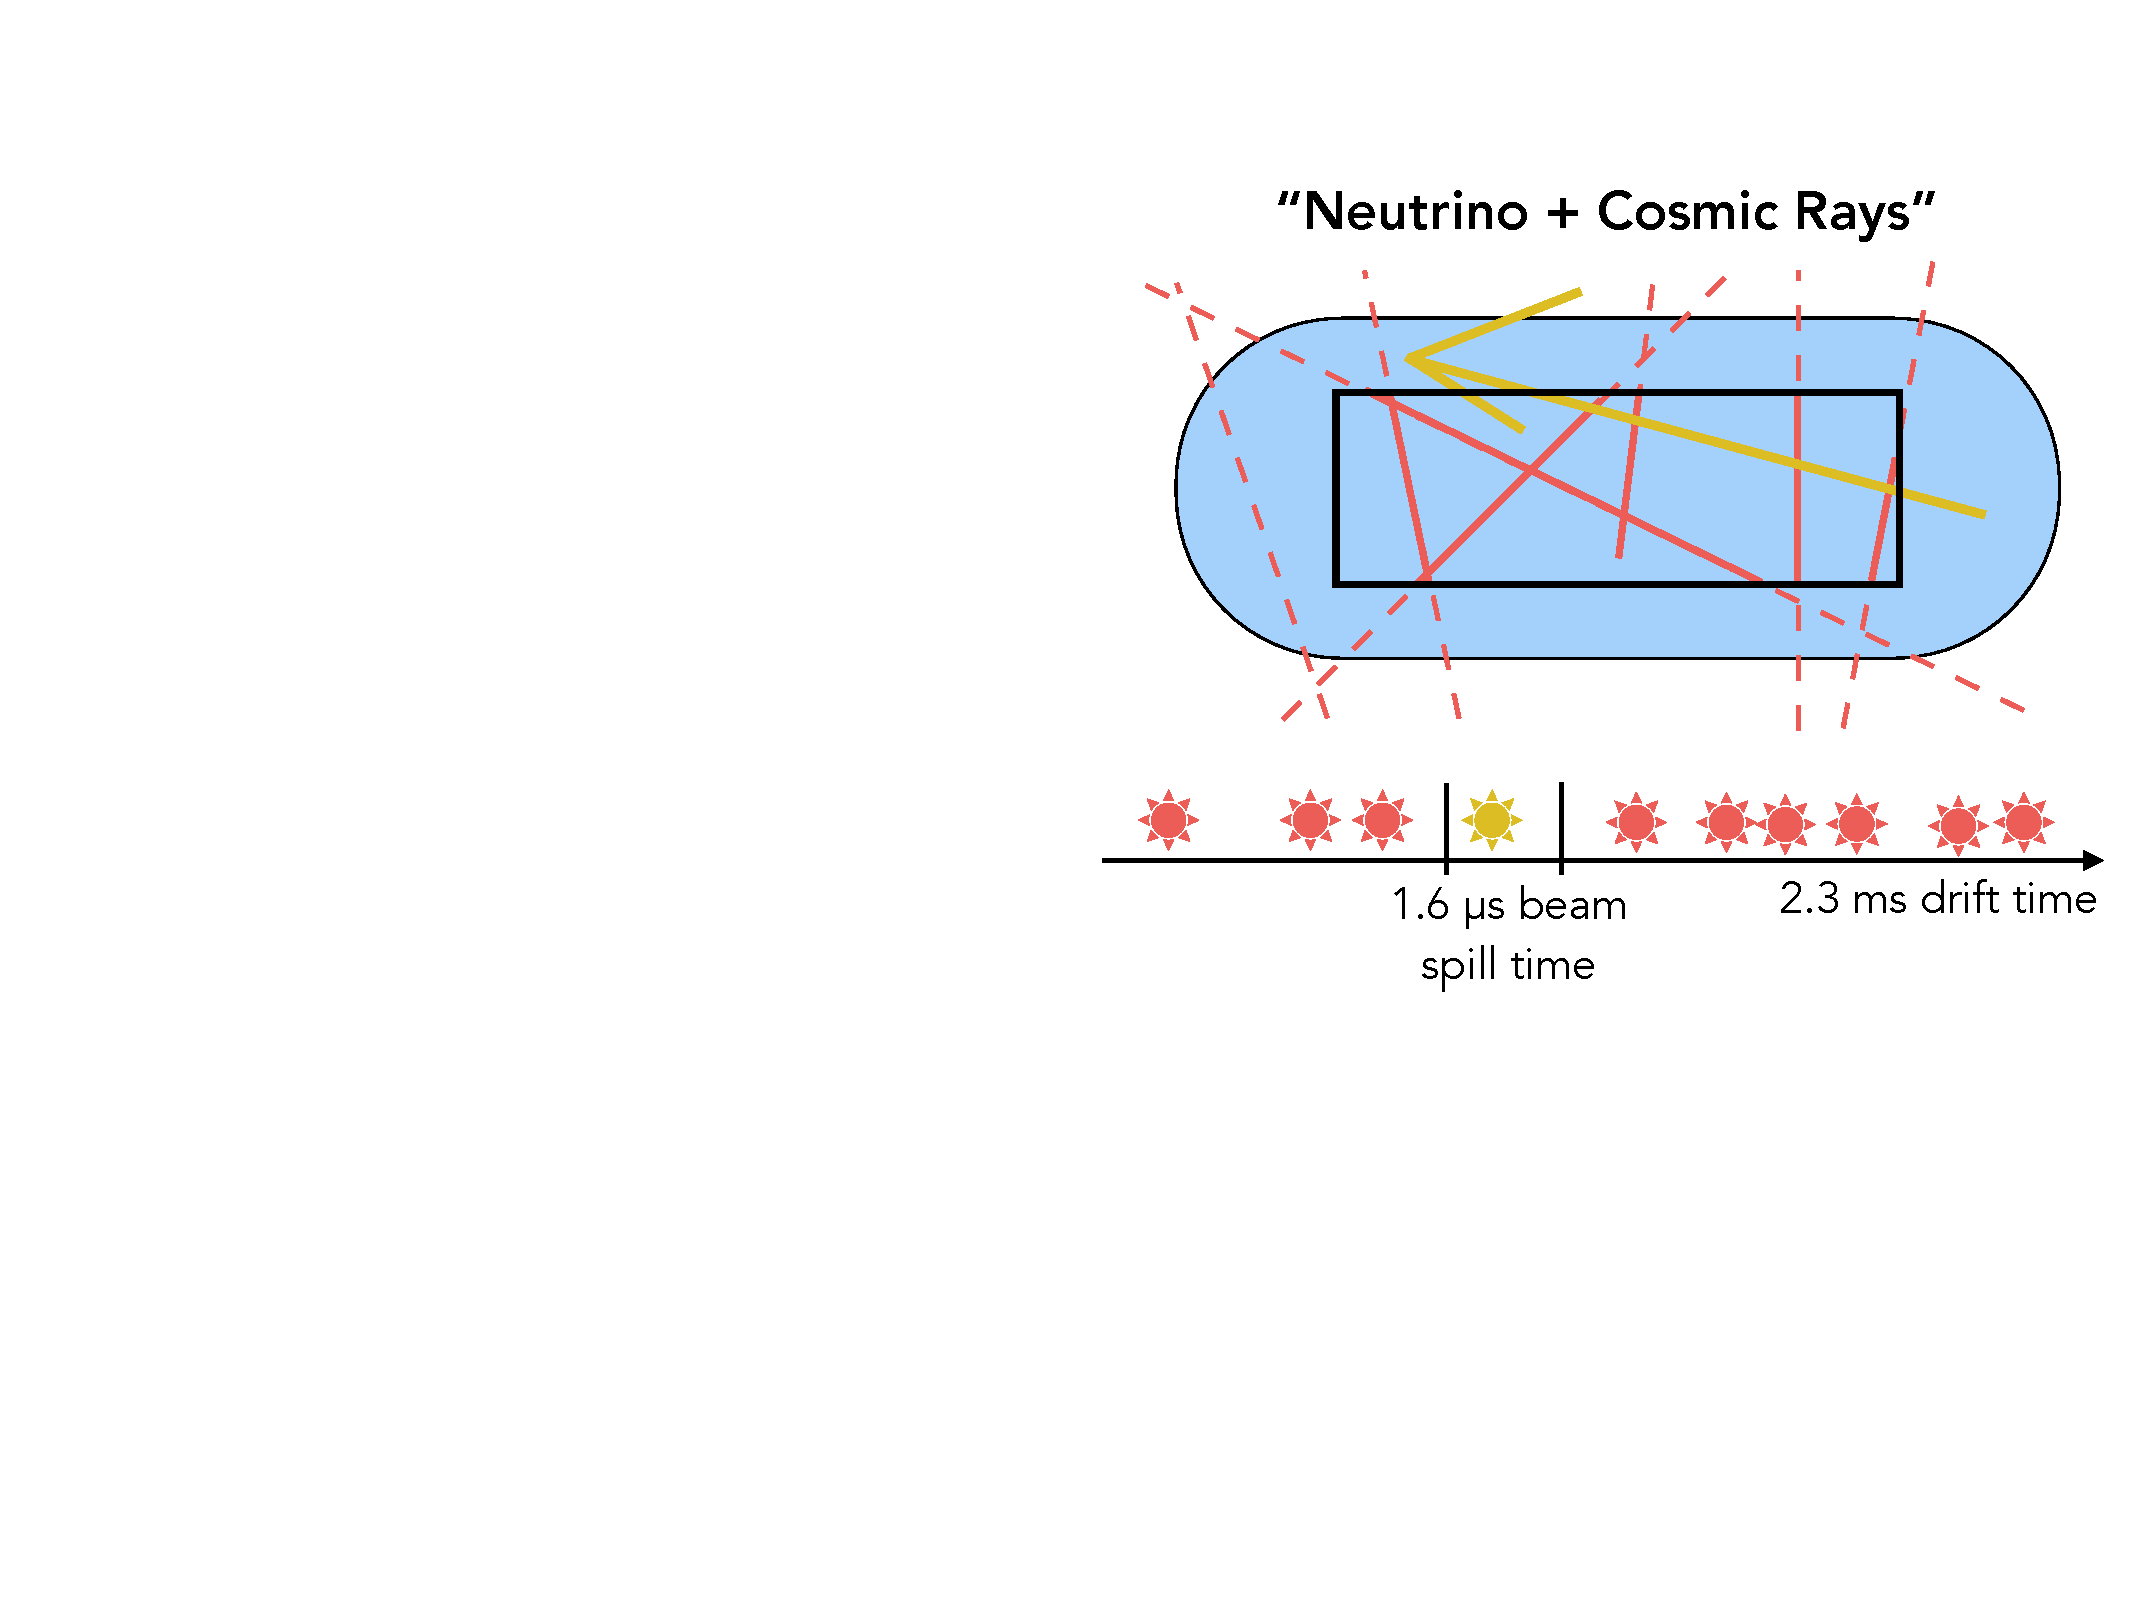
\includegraphics[width=.48\textwidth]{images/MicroBooNE/beam_on_beam_off_b}
   \label{fig:beam_on_beam_off_b}}
\caption[``Cosmic Rays Only'' and ``Neutrino + Cosmic Rays'' Event Examples]{Examples of a ``Cosmic Rays Only'' event~\protect\subref{fig:beam_on_beam_off_a}, where no neutrino interacted in the detector but one \acrshort{cr}s muon interacts during the beam spill window, triggering the detector readout, and of a ``Neutrino + Cosmic Rays'' event~\protect\subref{fig:beam_on_beam_off_b}, where a neutrino inetracts in the detector triggering the readout, but a \acrshort{cr} muon can still be selected instead of the neutrino origin muon track.}
\label{fig:beam_on_beam_off}
\end{figure}
%
\acrshort{cr}s are the dominant background in the analysis documented in this thesis, and this background is here divided into two categories, illustrated Figure~\ref{fig:beam_on_beam_off}: 
\begin{itemize}
\item recorded events where no neutrino interacted in the detector (Figure~\ref{fig:beam_on_beam_off_a}). These events can be estimated directly from data, by recording events when the neutrino beam is off. These events give rise to background events when one of the \acrshort{cr} muons interacts in the 1.6 $\mu$s beam time window producing a flash that triggers the system, and its topology fakes a neutrino interaction;
\item recorded events where one neutrino interacted in the detector (producing a flash that triggers the system) but a \acrshort{cr} muon is instead selected (Figure~\ref{fig:beam_on_beam_off_b}).
\end{itemize}
While the first background does not need to be simulated, as it can be estimated from data events when the neutrino beam is off, the second background needs to be simulated as a neutrino interaction is also present.
This is done using the COsmic Ray Simulations for KAscade (\textsc{Corsika}) generator \cite{corsika}. There are a variety of configurable parameters in \textsc{Corsika} including primary interaction particle type and low-energy hadronic models that are explored in detail in a MicroBooNE public note~\cite{corsika_note}. 
After both neutrino and \acrshort{cr} interactions have been simulated, the products of these interactions are ready to be tracked through the detector.

The simulation of the MicroBooNE detector is based on \textsc{Geant4}~\cite{geant} and includes particle propagation, drift of ionisation electrons to the wire planes, as well as propagation of scintillation light to the \acrshort{pmt}s.
Ionisation due to \acrshort{cr}s also leads to a distortion of the electric field within the detector. The effect is the build-up of slow-moving positive ions in a detector which gives rise to the so-called ``space charge'' effect~\cite{space_charge}. This effect leads to a displacement in the reconstructed position of signal ionisation electrons, as well as variations in the amount of charge quenching experienced by ionisation throughout the volume of the \acrshort{tpc}. The MicroBooNE detector simulation includes the space-charge effect.
All simulation is carried out within the LArSoft framework~\cite{larsoft}.

The work documented in this thesis uses two different configurations of \textsc{Genie}, summarised in Table~\ref{tab:genie_tunes}. The first one, which is the baseline configuration used in MicroBooNE, uses the default \textsc{Genie} configuration in which Fermi motion is described by the Bodek-Ritchie Fermi gas model~\cite{bodek_ritchie}, \acrshort{qe} and resonant pion production interactions are modelled according to the Llewellyn-Smith~\cite{llewellyn} and the Rein-Seghal~\cite{rein_sehgal} models respectively, and an additional term is added that enhances \acrshort{qe}-like interactions that occur off of correlated nucleon pairs via an empirically driven meson exchange current~\cite{mec_dytman}. The second, alternative configuration, includes the Valencia model for \acrshort{qe} interactions paired with a local Fermi gas model~\cite{nieves, nieves2} and Kuzmin-Lyubushkin-Naumov~\cite{kuzmin} and Berger-Sehgal model~\cite{berger_sehgal} for resonant pion production. The alternative configuration represents a theoretically driven set of models relevant at MicroBooNE energies.

\begin{table}[t]
\begin{adjustwidth}{-1cm}{-1cm}
\caption[\textsc{Genie} Model Configurations]{The two \g model sets used in the analysis presented in this thesis.}
\label{tab:genie_tunes}
\centering
\begin{tabular}{ccc}
\toprule
Model element & \tuneone & \tunethree  \\
\midrule
Nuclear Model              & Bodek-Ritchie Fermi Gas \cite{bodek_ritchie}  & Local Fermi Gas \cite{nieves, nieves2}  \\
Quasi-Elastic              & Llewellyn-Smith \cite{llewellyn}          & Nieves \cite{nieves, nieves2}  \\
Meson-Exchange Currents    & Empirical \cite{mec_dytman}               & Nieves \cite{nieves, nieves2} \\
Resonant                   & Rein-Seghal \cite{rein_sehgal}              & Berger-Seghal \cite{berger_sehgal} \\
Coherent                   & Rein-Seghal \cite{rein_sehgal}              & Berger-Seghal \cite{berger_sehgal} \\
\acrshort{fsi}                        & hA \cite{GENIE_reweighting}         & hA2014 \cite{GENIE_reweighting} \\
\bottomrule
\end{tabular}
\end{adjustwidth}
\end{table}

\section{Detector Operations}
\label{sec:detector_operations}

The MicroBooNE detector has been recording neutrino beam data since the fall of 2015. Figure~\ref{fig:run1} shows the amount of \acrfull{pot} collected since the start of operations. The \acrshort{cc} inclusive cross-section analysis presented in this thesis utilises $1.6 \times 10^{20}$ \acrshort{pot} of data (called ``Run 1''), collected from February to October 2016. More recent data, not used for the analysis in this thesis, benefits from the installation of a \acrshort{cr} tagger system~\cite{crt}. 

\begin{figure}[t]
\centering
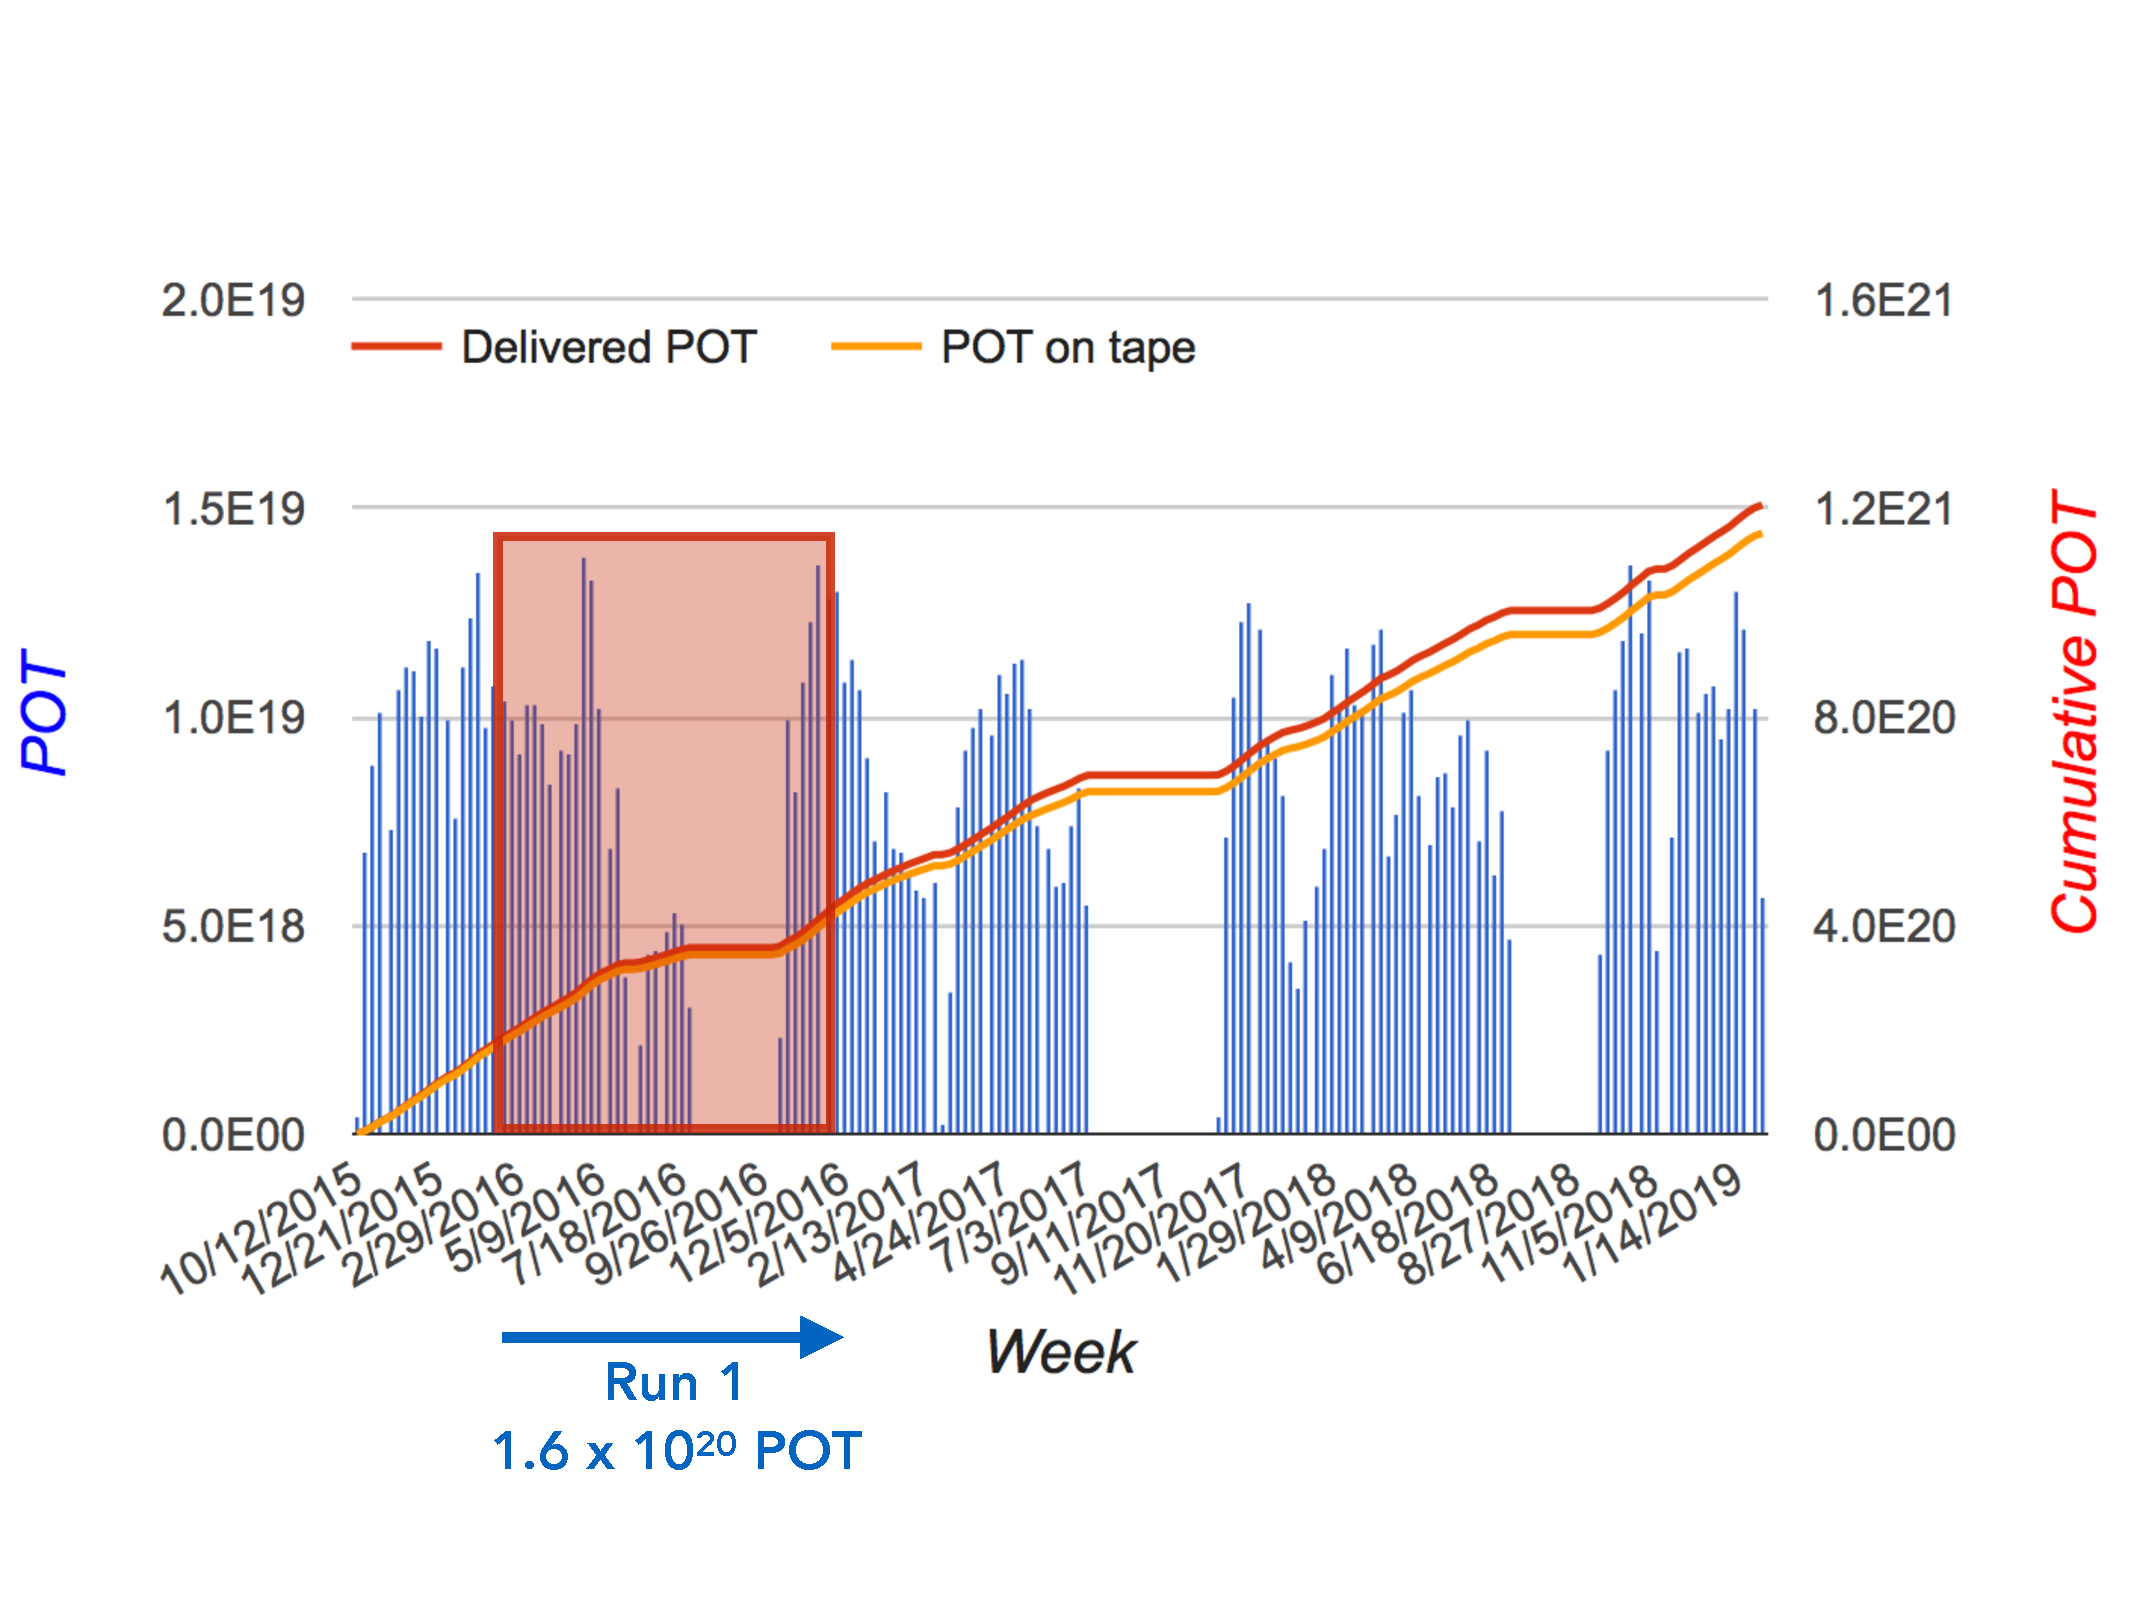
\includegraphics[width=0.85\textwidth]{images/MicroBooNE/run1}
\caption[Protons on Target over MicroBooNE Data-Taking Period]{Protons on target over MicroBooNE's two year data-taking period. Highlighted in red is the period used for the cross section analysis presented in this thesis.}
\label{fig:run1}
\end{figure}

